%%%%%%%%%%%%%%%%%%%%%%%%%%%%%%%%%%%%%%%%%%%%%%%%%%%%%%%%%%%%%%%%%%%%%%
% Overleaf (WriteLaTeX) Example: Molecular Chemistry Presentation
%
% Source: http://www.overleaf.com
%
% In these slides we show how Overleaf can be used with standard
% chemistry packages to easily create professional presentations.
%
% Feel free to distribute this example, but please keep the referral
% to overleaf.com
%
%%%%%%%%%%%%%%%%%%%%%%%%%%%%%%%%%%%%%%%%%%%%%%%%%%%%%%%%%%%%%%%%%%%%%%

\documentclass[xcolor={dvipsnames}]{beamer}

\mode<presentation>
{
  \usetheme{Madrid}       % or try default, Darmstadt, Warsaw, ...
  \usecolortheme{default} % or try albatross, beaver, crane, ...
  \usefonttheme{default}    % or try default, structurebold, ...
  \setbeamertemplate{navigation symbols}{}
  \setbeamertemplate{caption}[numbered]
}

\usepackage[english]{babel}
\usepackage[utf8x]{inputenc}
\usepackage{graphicx}
\usepackage{hyperref}
  \hypersetup{colorlinks=true}
  \hypersetup{urlcolor=blue}
  \hypersetup{linkcolor = .}
\usepackage{xcolor}
\usepackage{siunitx}
  \sisetup{separate-uncertainty = true}
\DeclareSIUnit\barn{b}
\usepackage{physics}
\usepackage[font=small,labelfont=bf]{caption}
\usepackage{subcaption}
\usepackage[en-GB]{datetime2}
\usepackage{overpic}
\usepackage{feynmp}
\DeclareGraphicsRule{*}{mps}{*}{}
\usepackage{scalerel}
\newcommand{\mylbrace}[2]{\vspace{#2pt}\hspace{6pt}\scaleleftright[\dimexpr5pt+#1\dimexpr0.06pt]{\lbrace}{\rule[\dimexpr2pt-#1\dimexpr0.5pt]{-4pt}{#1pt}}{.}}
\newcommand{\myrbrace}[2]{\vspace{#2pt}\scaleleftright[\dimexpr5pt+#1\dimexpr0.06pt]{.}{\rule[\dimexpr2pt-#1\dimexpr0.5pt]{-4pt}{#1pt}}{\rbrace}\hspace{6pt}}

% Trim in percent
\usepackage{adjustbox}

% No "Figure" prefix
\setbeamertemplate{caption}{\raggedright\insertcaption\par}

% Nice decay amplitude diagrams
\usepackage{amsmath,amssymb,tikz-cd}

% Strike out text
\usepackage[normalem]{ulem}

% For figures with text overlay
\usepackage{overpic}

% Arrows
\usepackage{tikz}
\newcommand{\tikzmark}[1]{\tikz[remember picture] \node[coordinate] (#1) {#1};}

% Colourbox with line breaks
\newcommand{\cbox}[2][lime!20]{%
  \colorbox{#1}{\parbox{\dimexpr\linewidth-2\fboxsep}{\strut #2\strut}}%
}

% Vector arrows
\usepackage[pdftex]{pict2e}

% Checkmark symbol
\def\checkmark{\tikz\fill[scale=0.4](0,.35) -- (.25,0) -- (1,.7) -- (.25,.15) -- cycle;}

% Copy code
\usepackage{listings}
\lstset{
  basicstyle=\ttfamily\tiny,
  breaklines=true
}

% Definitions from Fabian
\usepackage{xspace}
\usepackage{booktabs}
\def\pip    {{\ensuremath{\pi^+}}\xspace}
\def\pim    {{\ensuremath{\pi^-}}\xspace}
\def\Kp     {{\ensuremath{K^+}}\xspace}
\def\Km     {{\ensuremath{K^-}}\xspace}
\def\Dz     {{\ensuremath{D^0}}\xspace}
\def\DKpi   {\ensuremath{\Dz \rightarrow \Km \pip}\xspace}     
\def\DKpipipi   {\ensuremath{\Dz \rightarrow \Km \pip \pip \pim}\xspace} 

% Here's where the presentation starts, with the info for the title slide
\title[RTA WP4 meeting]{Update on 2026 tracking efficiencies}

\author[Martin Tat]{Rowina Caspary$^1$, Michel De Cian$^2$, Fabian Glaser$^1$, Stephanie Hansmann-Menzemer$^1$, Peilian Li$^3$, Maurice Morgenthaler$^1$, \\ \textbf{Martin Tat}$^1$}
\institute[Heidelberg]{Heidelberg University$^1$, University of Manchester$^2$, UCAS$^3$}
\date{8th October 2026}

\titlegraphic{
\includegraphics[height = 1.2cm]{../lhcb.jpg}\hspace{1.0cm}~%
              
\includegraphics[height = 1.2cm]{../FSP_logo.png}
              
\includegraphics[height = 1.2cm]{../ManchesterLogo.jpg}~%
              
\includegraphics[height = 1.2cm]{../UCAS_logo.png}~%
              
\includegraphics[height = 1.2cm]{../HeidelbergLogo.pdf}}

\begin{document}

\begin{frame}
  \titlepage
\end{frame}

% These three lines create an automatically generated table of contents.
%\begin{frame}{Outline}
%  \tableofcontents
%\end{frame}

\begin{frame}{Tag-and-probe method}
  \vspace{0.0cm}
  \begin{figure}[htb]
    \centering
    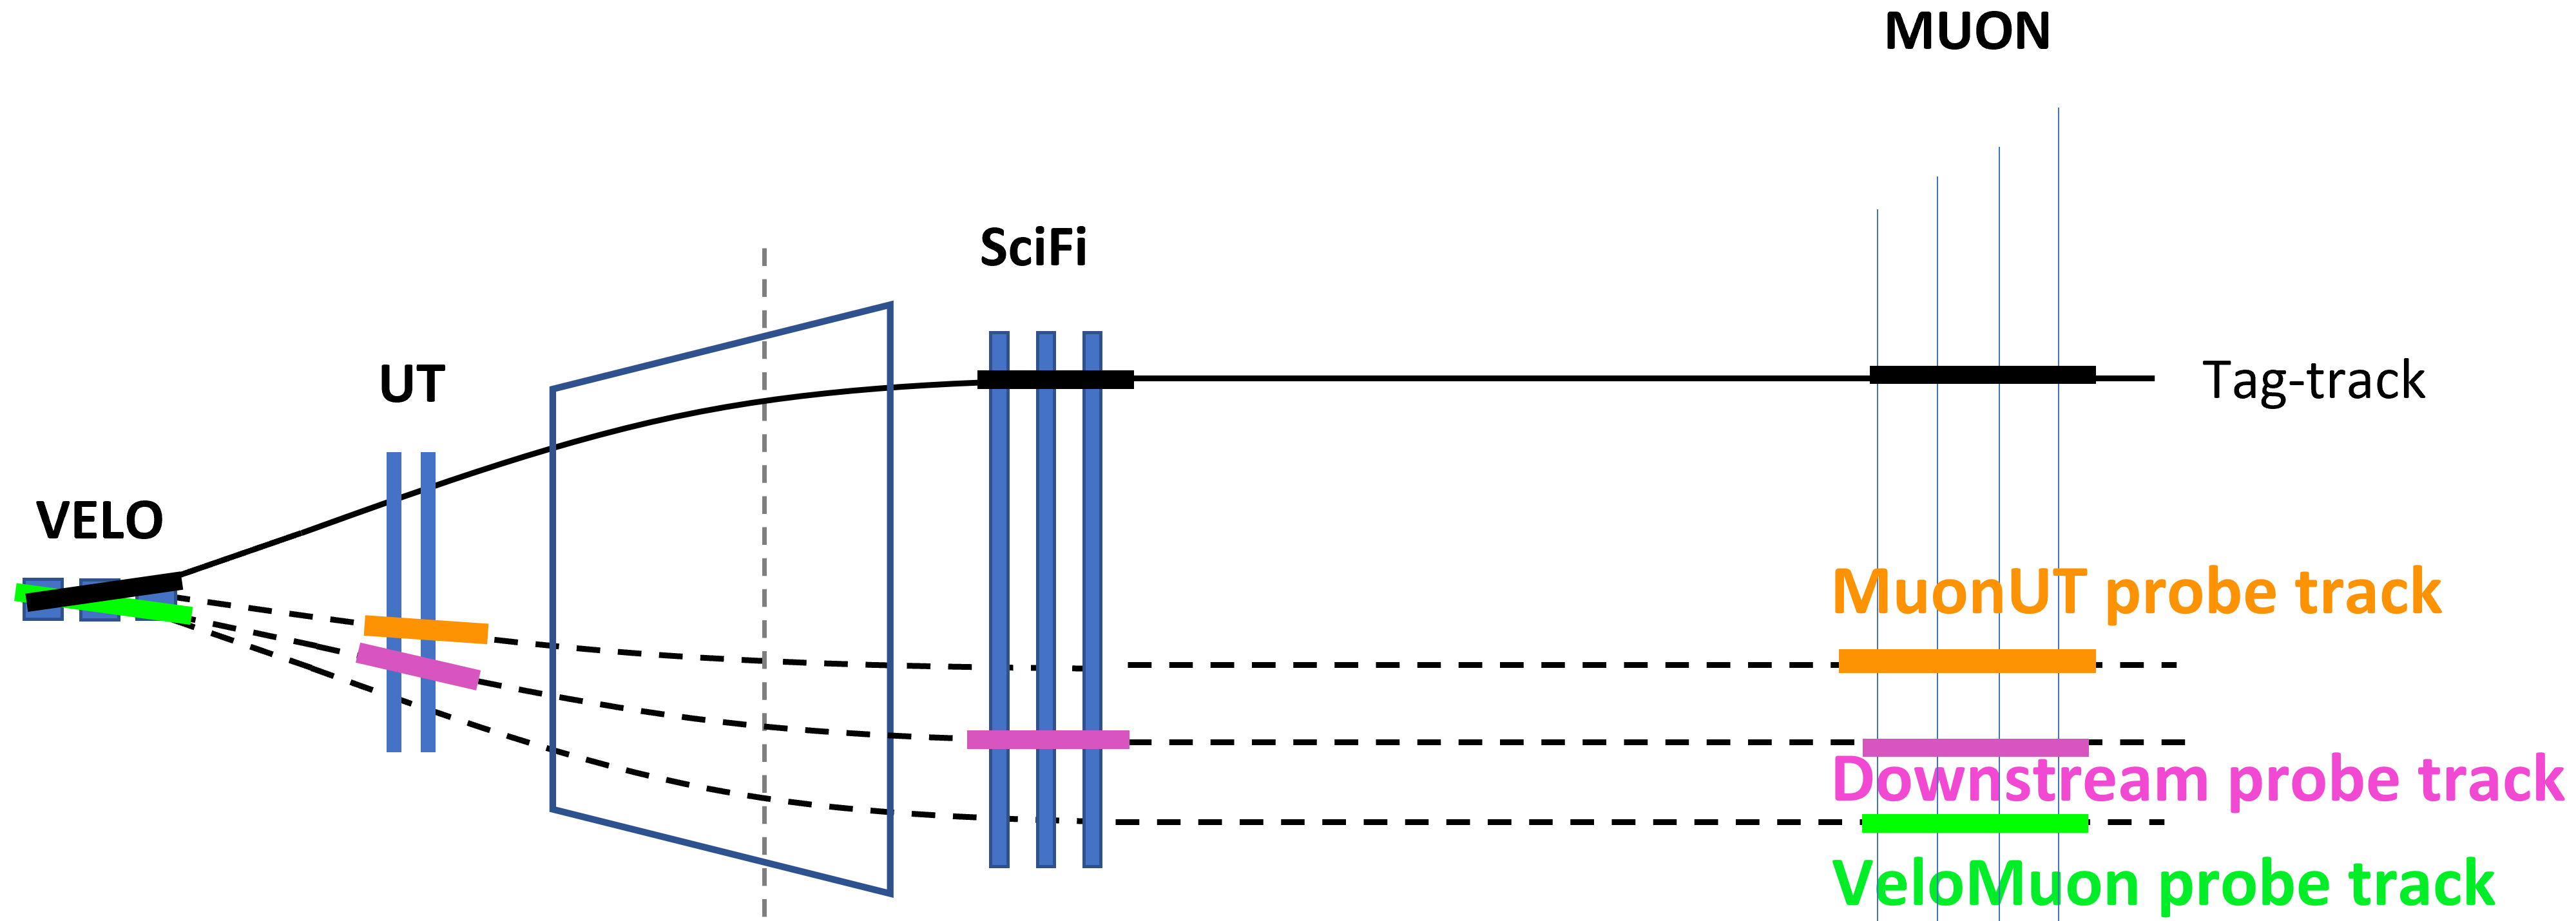
\includegraphics[width=0.75\textwidth]{Plots/Tag_and_probe_method.png}
    \caption*{\tiny Figure by Rowina}
  \end{figure}
  \vspace{-0.1cm}
  \begin{itemize}
    \item{Tag-and-probe method with $J/\psi\to\mu^+\mu^-$}
    \item{Fully reconstruct one muon...}
    \item{... and partially reconstruct the other muon}
    \item{Match hits in specific sub-detector with partially reconstructed track}
  \end{itemize}
  \begin{equation*}
    \epsilon_{\rm track} = \frac{N_{\rm matched}}{N_{\rm matched} + N_{\rm failed}}
  \end{equation*}
\end{frame}

\begin{frame}{Introduction to methods}
  \vspace{0.0cm}
  {\Large Strategy for tracking efficiency determination:}
  \vspace{0.2cm}
  \begin{itemize}
    \setlength\itemsep{0.8em}
    \item{Combine efficiencies of two methods:}
    \begin{itemize}
      \item{VeloMuon: SciFi efficiency}
      \item{Downstream: Velo efficiency}
      \item{Combined: Velo $\times$ SciFi efficiencies}
    \end{itemize}
    \item{Cross check with long track efficiency from the MuonUT method}
    \begin{itemize}
      \item{Main systematic}
    \end{itemize}
  \end{itemize}
\end{frame}

\begin{frame}{Overview of work}
  \vspace{0.0cm}
  {Information for analysts:}
  \vspace{0.2cm}
  \begin{itemize}
    \setlength\itemsep{0.5em}
    \item{v0 tables available on GitLab \href{https://gitlab.cern.ch/lhcb-rta/tracking-efficiencies-run-3}{here}}
    \item{Muon tracking efficiency corrections and hadronic corrections}
    \item{Currently preliminary tables are available for 2024 and 2025}
    \item{Note: Hadronic corrections just updated, plan to present next week}
  \end{itemize}
  \vspace{0.5cm}
  {Tracking efficiencies are determined using TrackCalib2}
  \vspace{0.2cm}
  \begin{itemize}
    \setlength\itemsep{0.5em}
    \item{GitLab repository \href{https://gitlab.cern.ch/lhcb-rta/trackcalib2}{here}}
    \item{Mass fit done on tuples from AP to extract efficiencies}
    \item{Note: Analysts should \underline{not} have to run TrackCalib2 themselves, unless the released numbers are not suitable (need different binning, etc)}
  \end{itemize}
\end{frame}

\begin{frame}{2026 datasets}
  \vspace{0.0cm}
  {\large Today I will present 2026 tracking efficiencies:}
  \vspace{0.2cm}
  \begin{itemize}
    \setlength\itemsep{1.0em}
    \item{Note: \underline{Expected} 2026 MC is used}
    \item{Split into blocks by sprucing campaign}
    \begin{itemize}
      \item[-]{Block 1: Sprucing26c1 MagDown}
      \item[-]{Block 2: Sprucing26c1 MagUp}
      \item[-]{Block 3: Sprucing26c1 MagDown}
      \item[-]{Block 4: Sprucing26c1 MagUp}
    \end{itemize}
  \end{itemize}
\end{frame}

\begin{frame}{2026 tracking efficiencies}
  \vspace{0.0cm}
  {\large Comparison of tracking efficiencies in 2026 data blocks}
  \begin{figure}[htb]
    \centering
    \begin{subfigure}{0.5\textwidth}
      \centering
      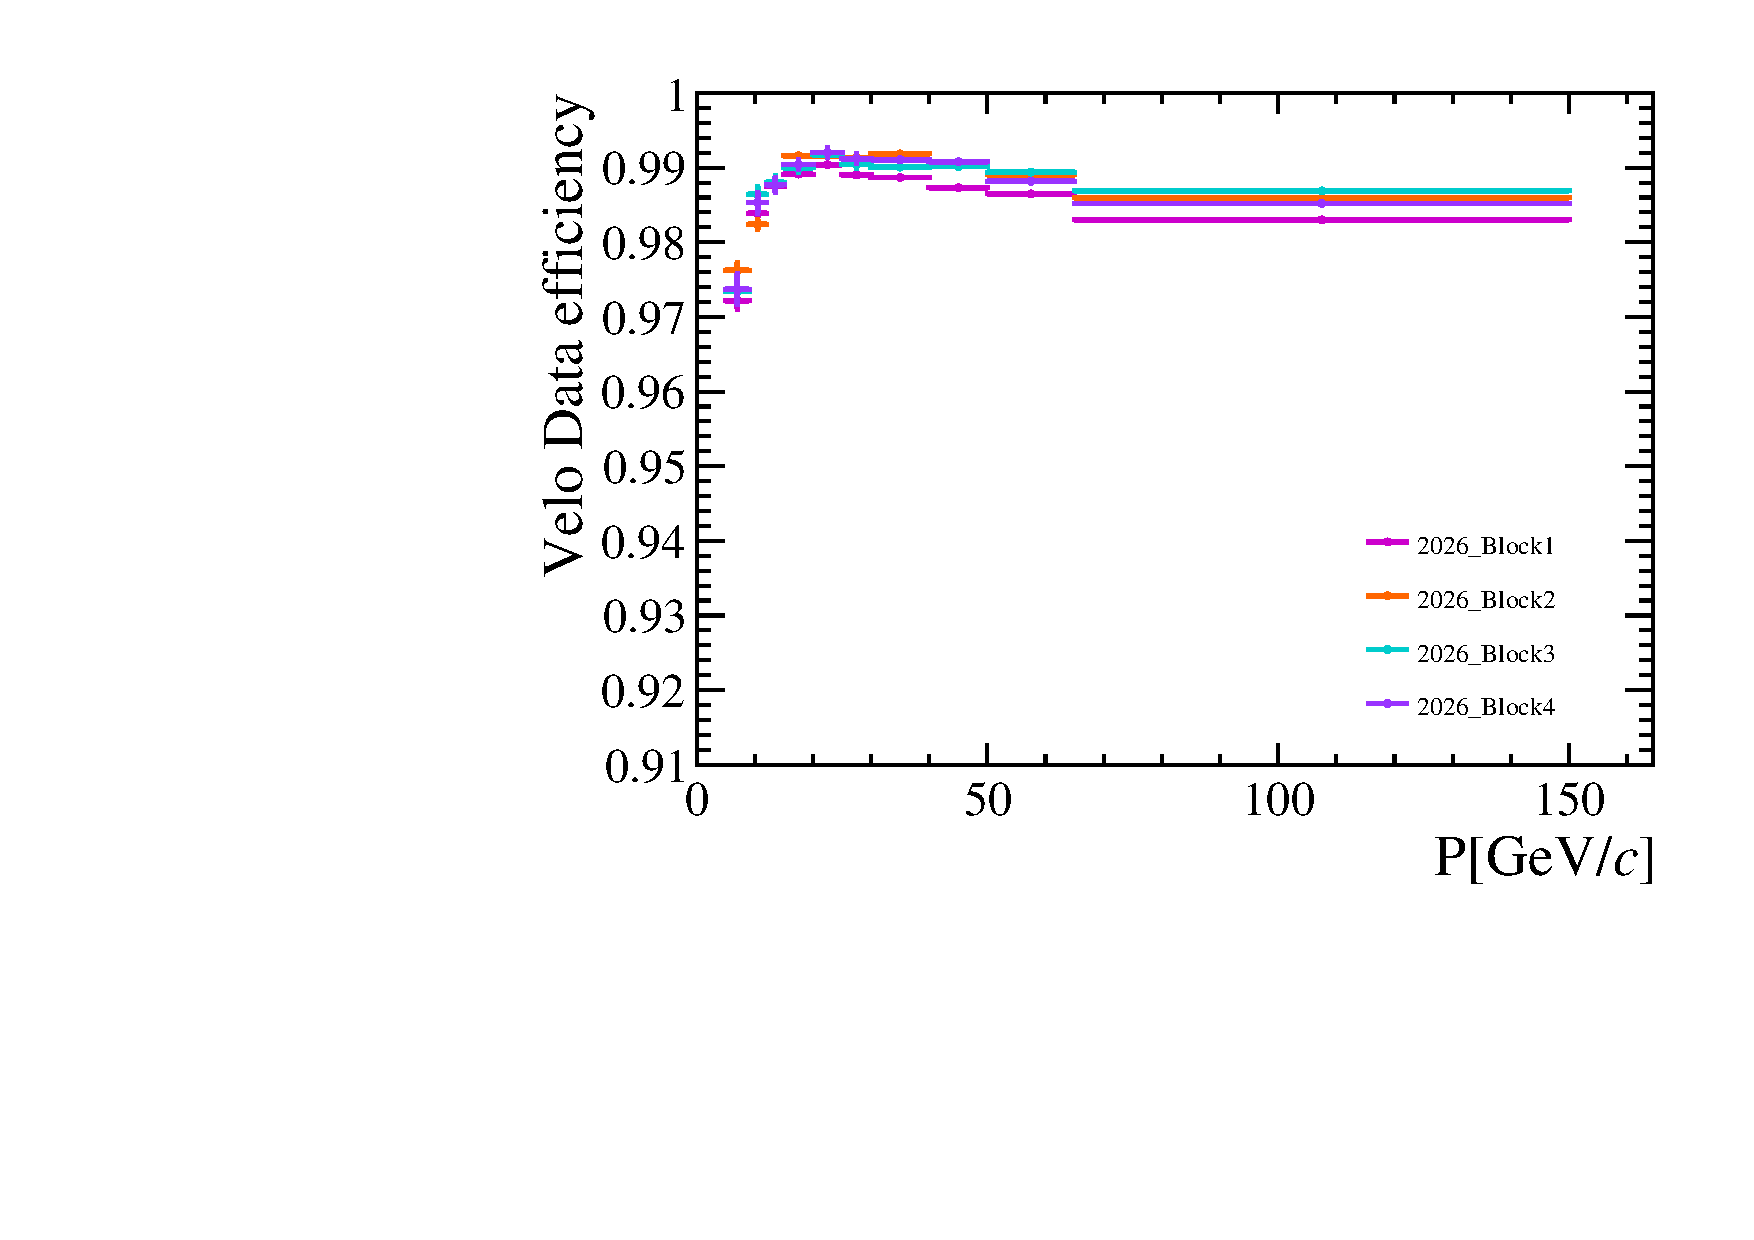
\includegraphics[width=1.0\textwidth]{Plots/trackeff_Data_Downstream_P_2026_expected_MC_samples.pdf}
    \end{subfigure}%
    \begin{subfigure}{0.5\textwidth}
      \centering
      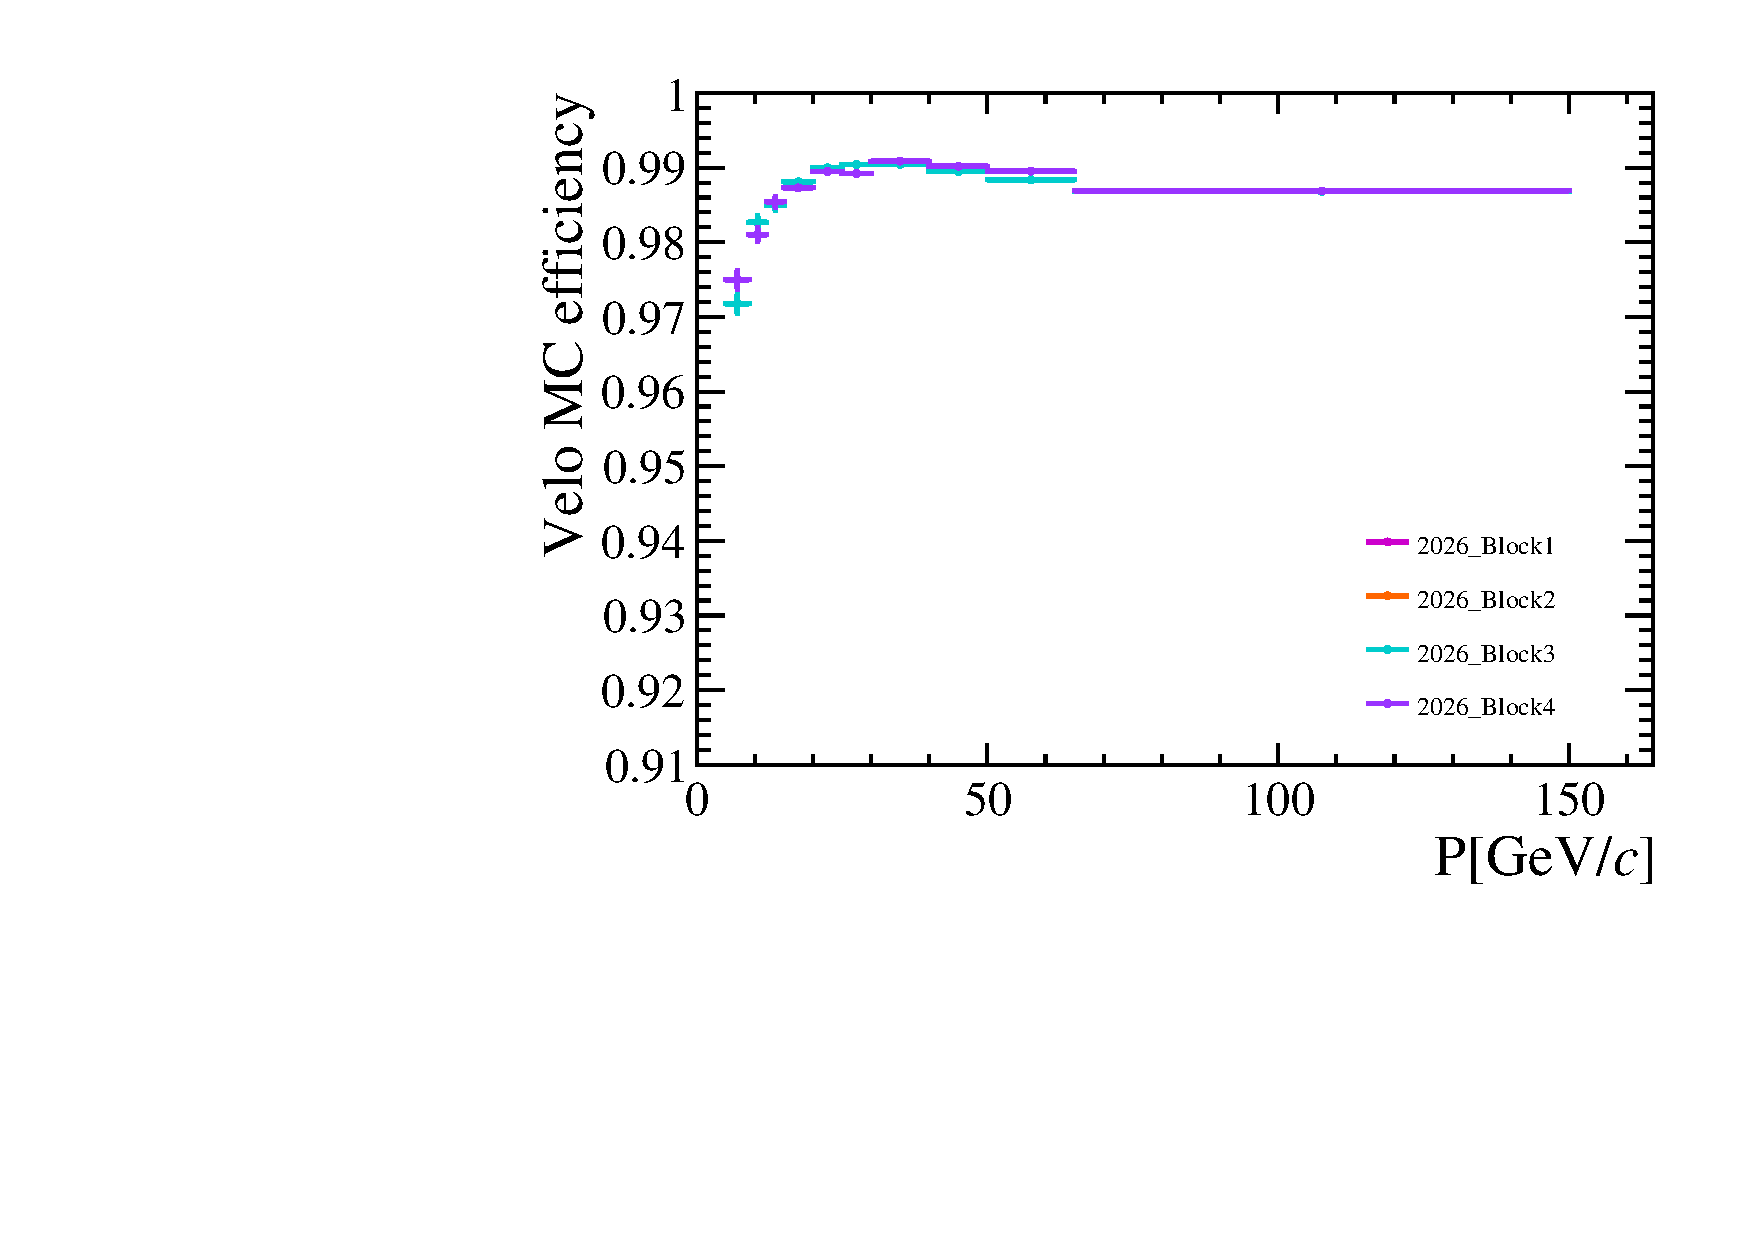
\includegraphics[width=1.0\textwidth]{Plots/trackeff_MC_Downstream_P_2026_expected_MC_samples.pdf}
    \end{subfigure}
  \end{figure}
  {Velo efficiencies agree reasonably well between data and MC in $p$...}
\end{frame}

\begin{frame}{2026 tracking efficiencies}
  \vspace{0.0cm}
  {\large Comparison of tracking efficiencies in 2026 data blocks}
  \begin{figure}[htb]
    \centering
    \begin{subfigure}{0.5\textwidth}
      \centering
      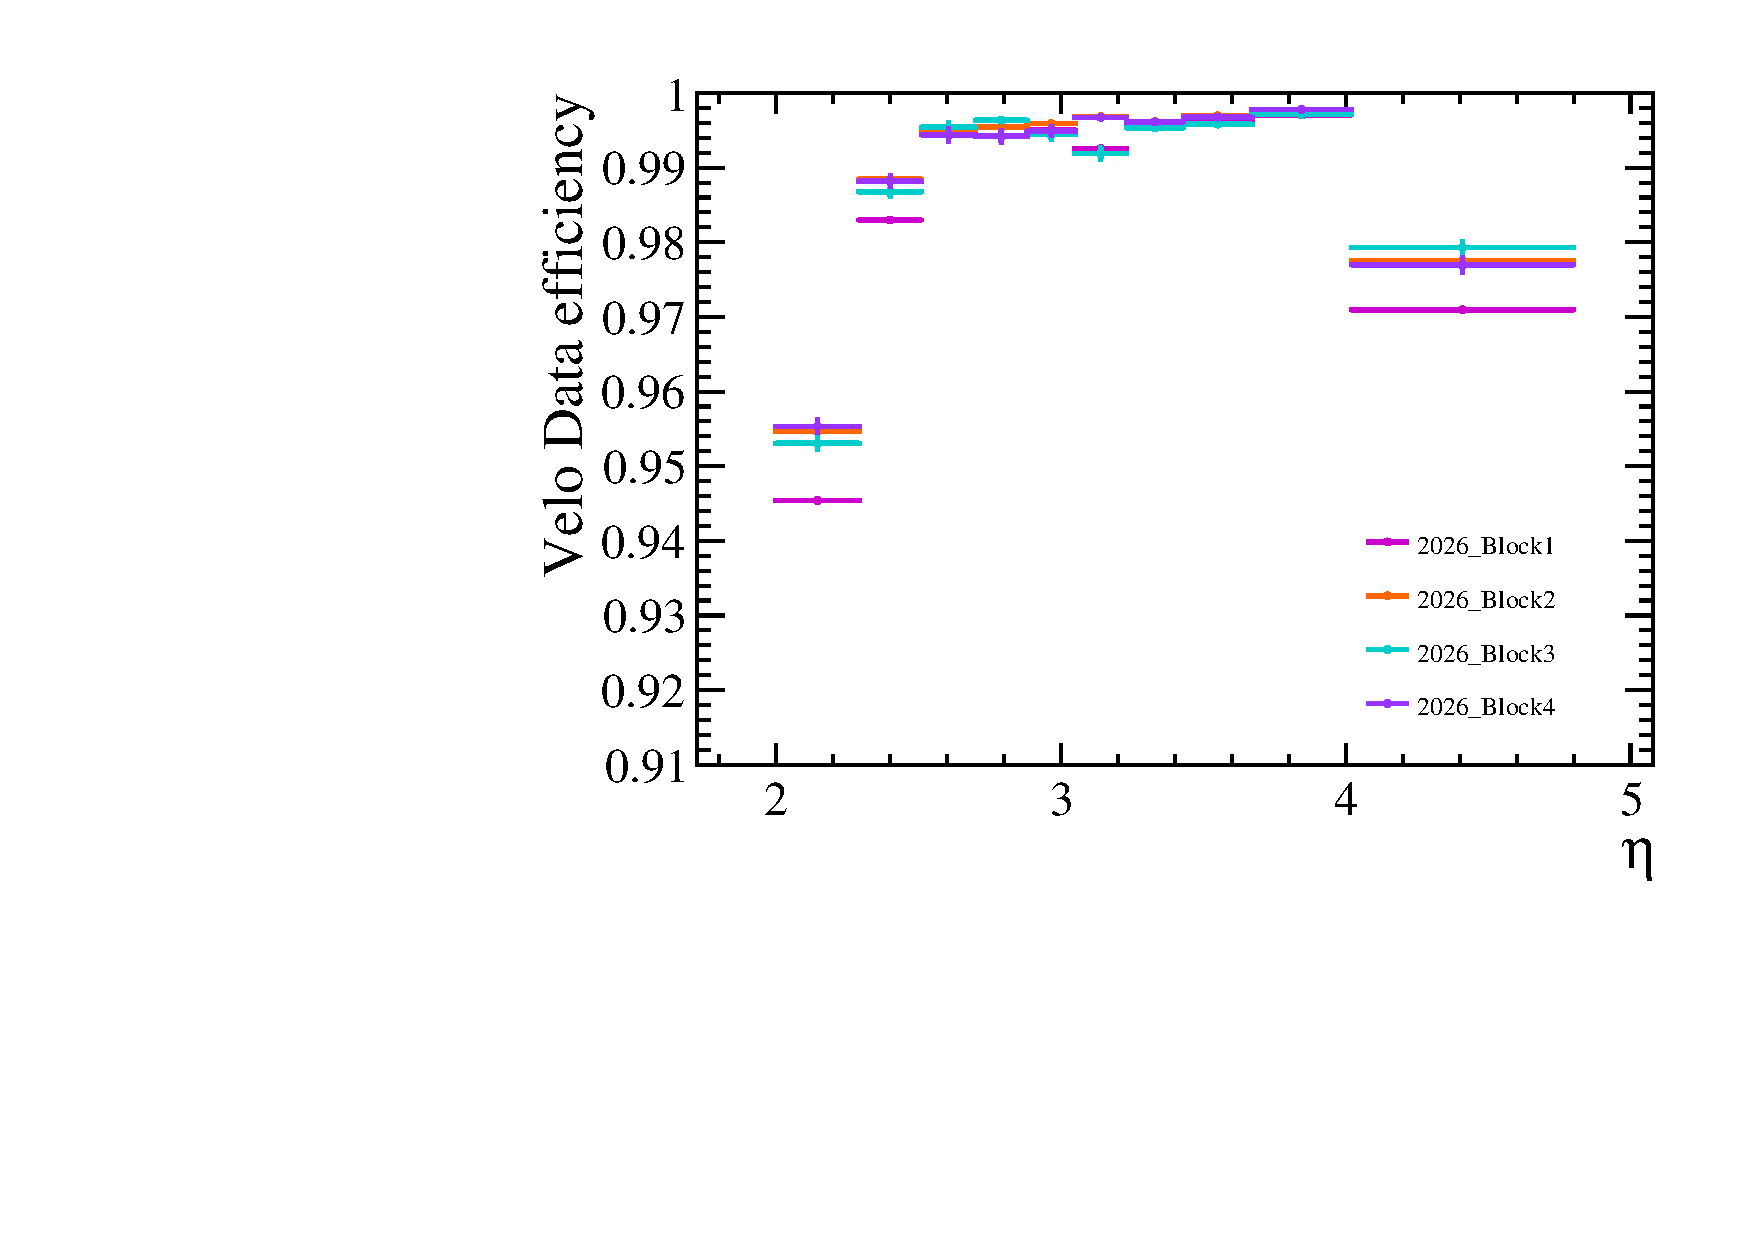
\includegraphics[width=1.0\textwidth]{Plots/trackeff_Data_Downstream_ETA_2026_expected_MC_samples.pdf}
    \end{subfigure}%
    \begin{subfigure}{0.5\textwidth}
      \centering
      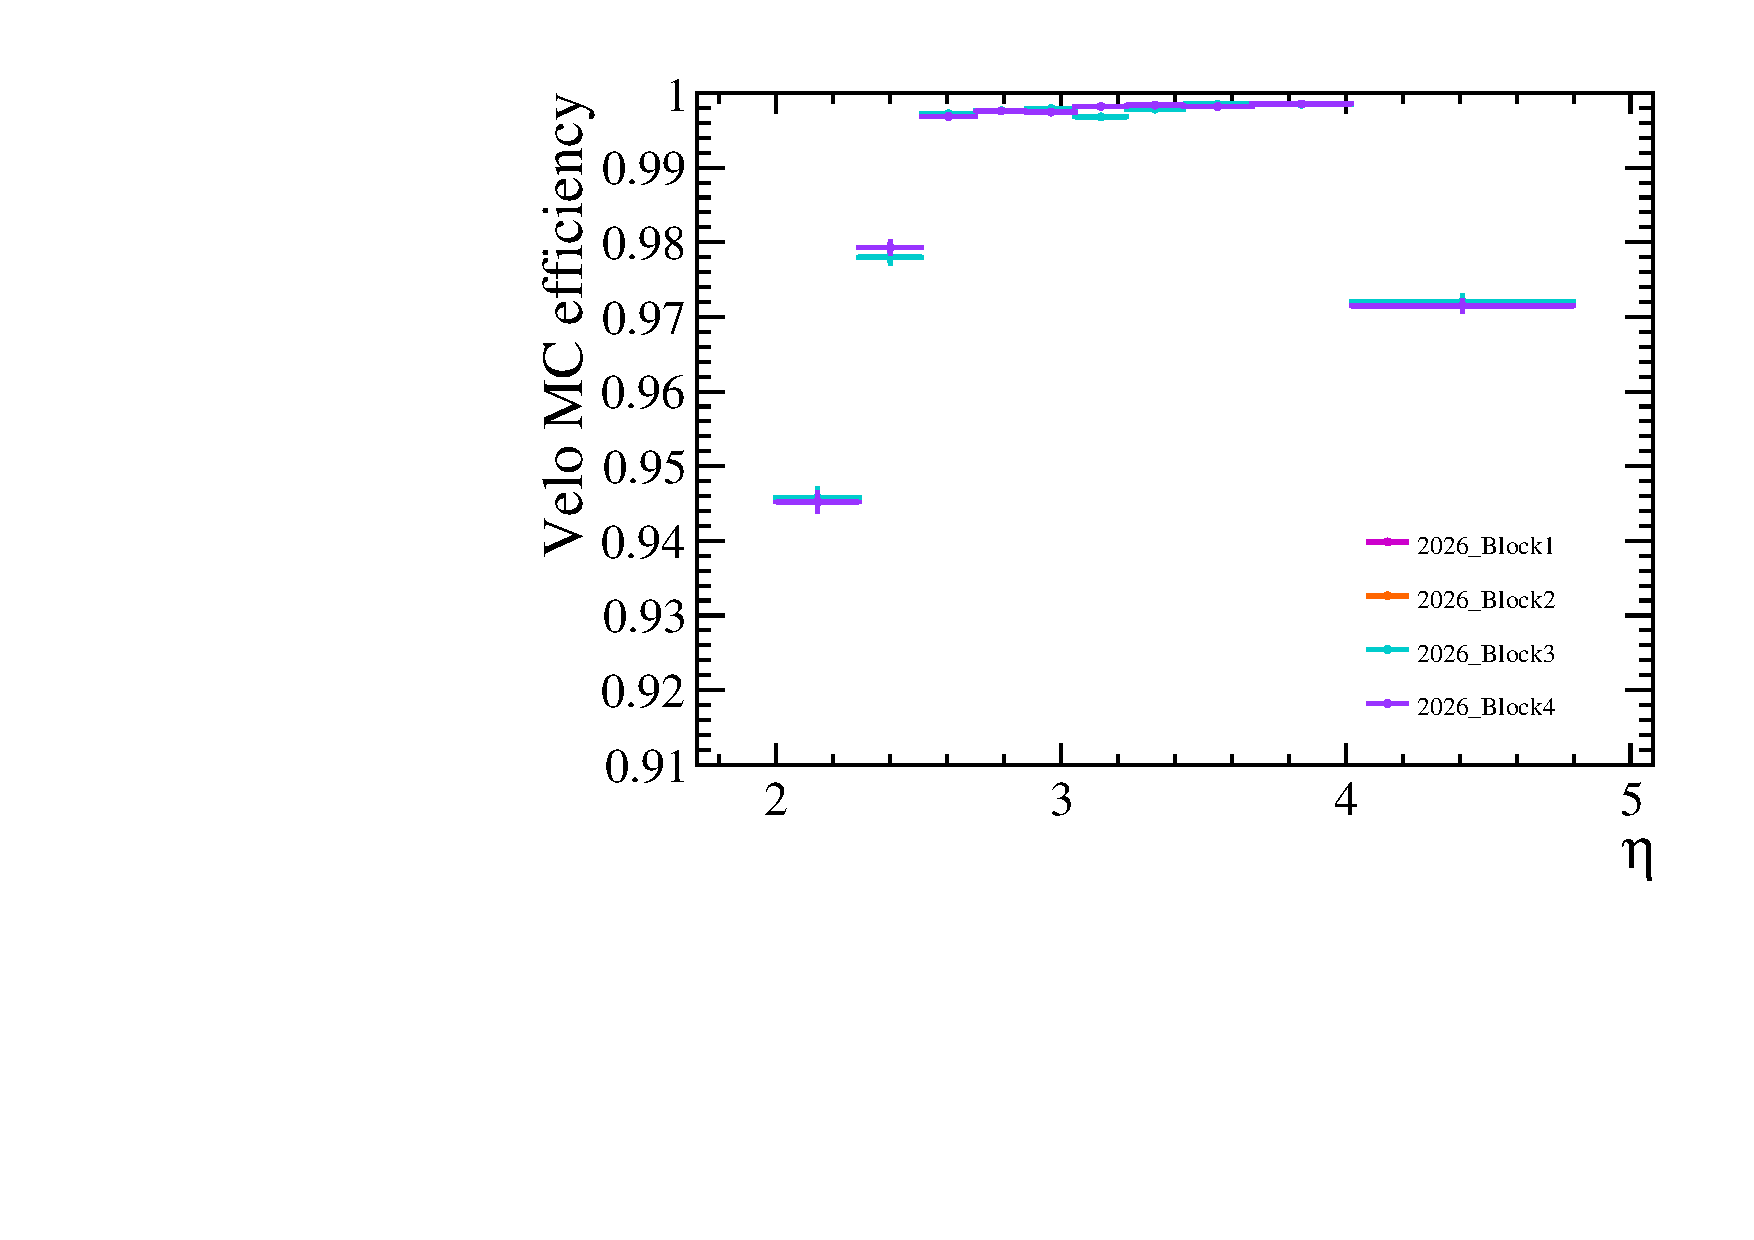
\includegraphics[width=1.0\textwidth]{Plots/trackeff_MC_Downstream_ETA_2026_expected_MC_samples.pdf}
    \end{subfigure}
  \end{figure}
  {... but in $\eta$ some features are seen at low and high $\eta$ after 2026 Block 1}
\end{frame}

\begin{frame}{Velo changes during data taking}
  \vspace{0.0cm}
  \begin{itemize}
    \item{It's unclear why the Velo efficiencies are higher in Blocks 2, 3, 4}
    \item{Magnet flip happened on 25th March 2026}
    \item{From Run meeting Velo minutes on 20th March 2026:}
    \begin{itemize}
      \item[-]{\textit{``Tuesday. HV recipes updated. STANDBY2 with 400V for inner sensors and 200V for outer sensors. M30 VP2 with 600V at ready''}}
    \end{itemize}
    \item{From Run meeting Velo minutes on 24th March 2026:}
    \begin{itemize}
      \item[-]{\textit{``HV recipes updated with M30/M31 VP2 and VP0 at 600V''}}
      \item[-]{\textit{``... After some investigation, M30 VP2-0 was confirmed to be damaged. HV recipes rollback to 400V inner sensors and 200V outer sensors.''}}
    \end{itemize}
    \item{Furthermore, several ASICs failed during this period...}
    \item{... but change in HV could explain the higher efficiencies}
  \end{itemize}
\end{frame}

\begin{frame}{2026 tracking efficiencies}
  \vspace{0.0cm}
  {\large Comparison of tracking efficiencies in 2026 data blocks}
  \begin{figure}[htb]
    \centering
    \begin{subfigure}{0.5\textwidth}
      \centering
      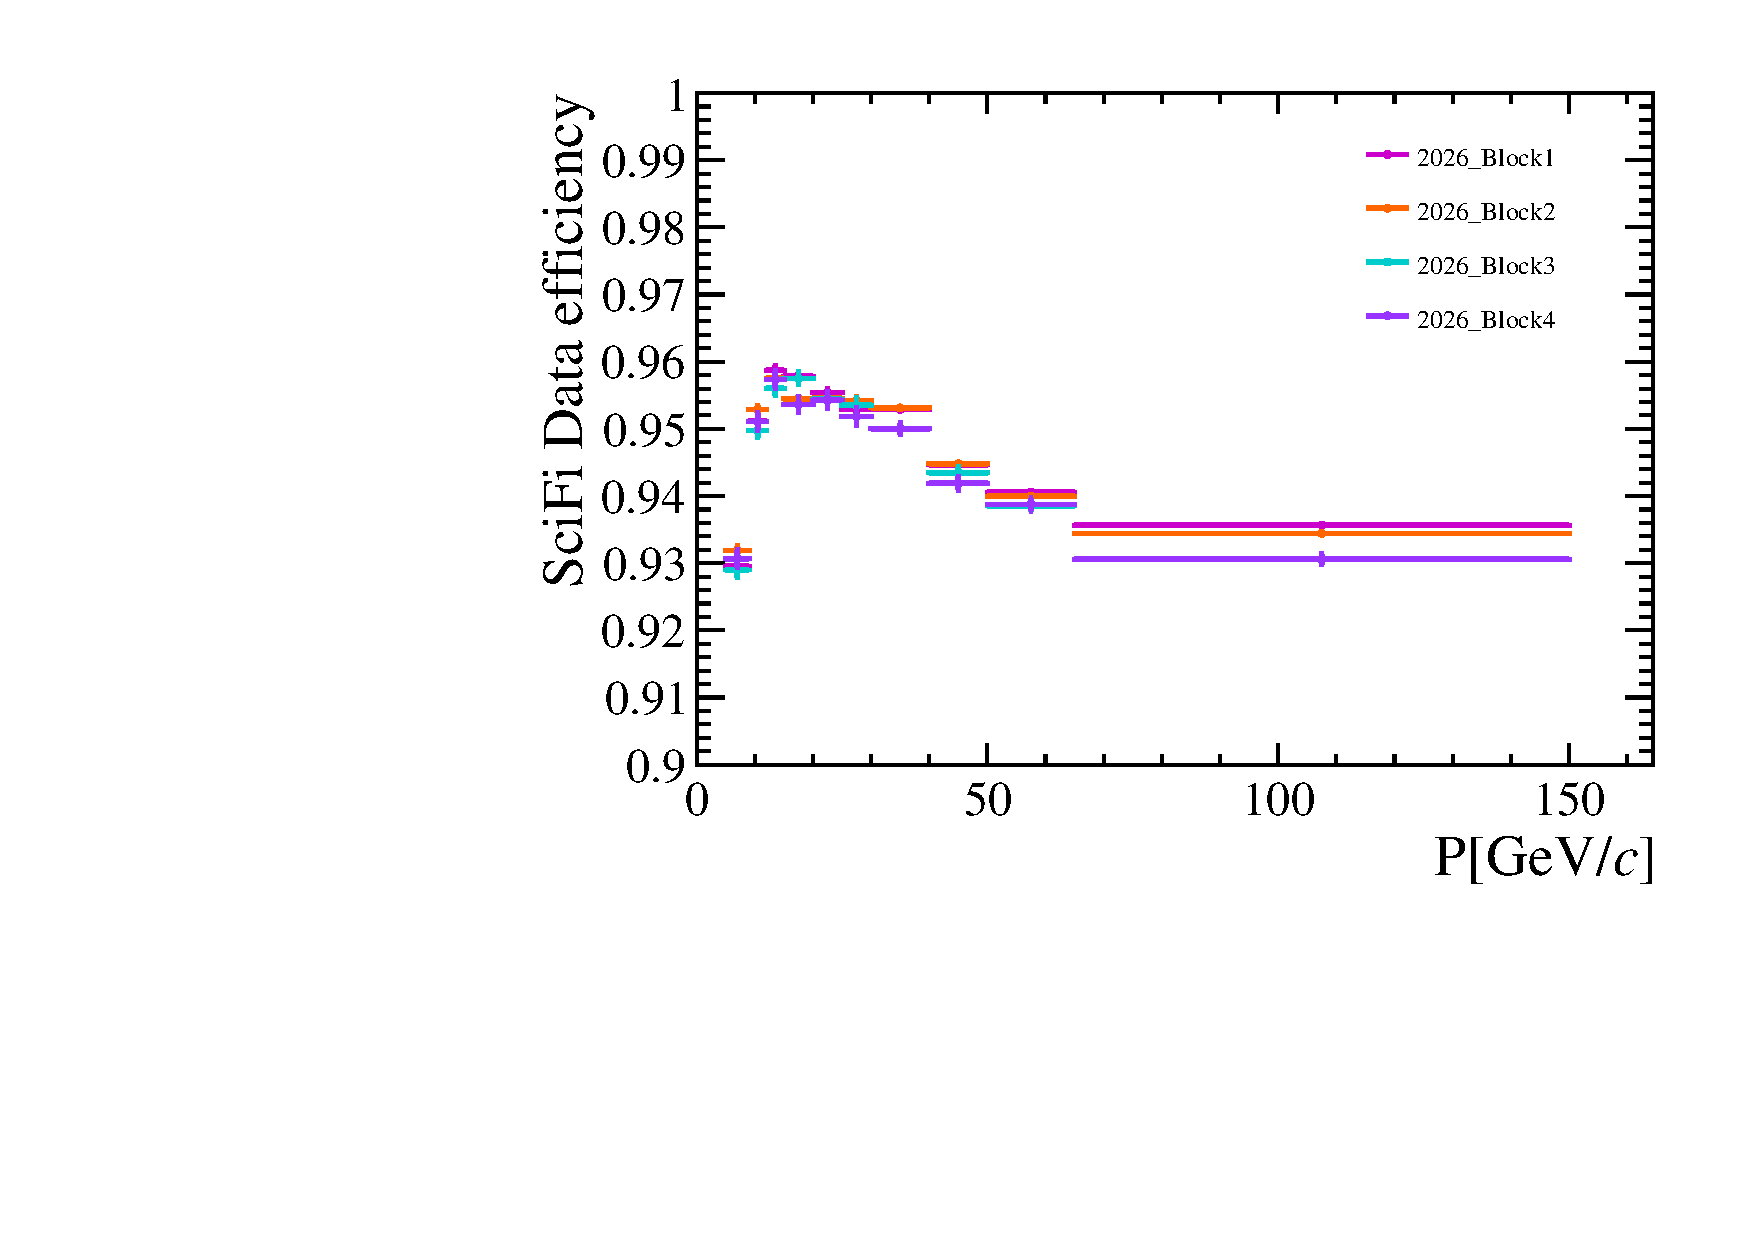
\includegraphics[width=1.0\textwidth]{Plots/trackeff_Data_VeloMuon_P_2026_expected_MC_samples.pdf}
    \end{subfigure}%
    \begin{subfigure}{0.5\textwidth}
      \centering
      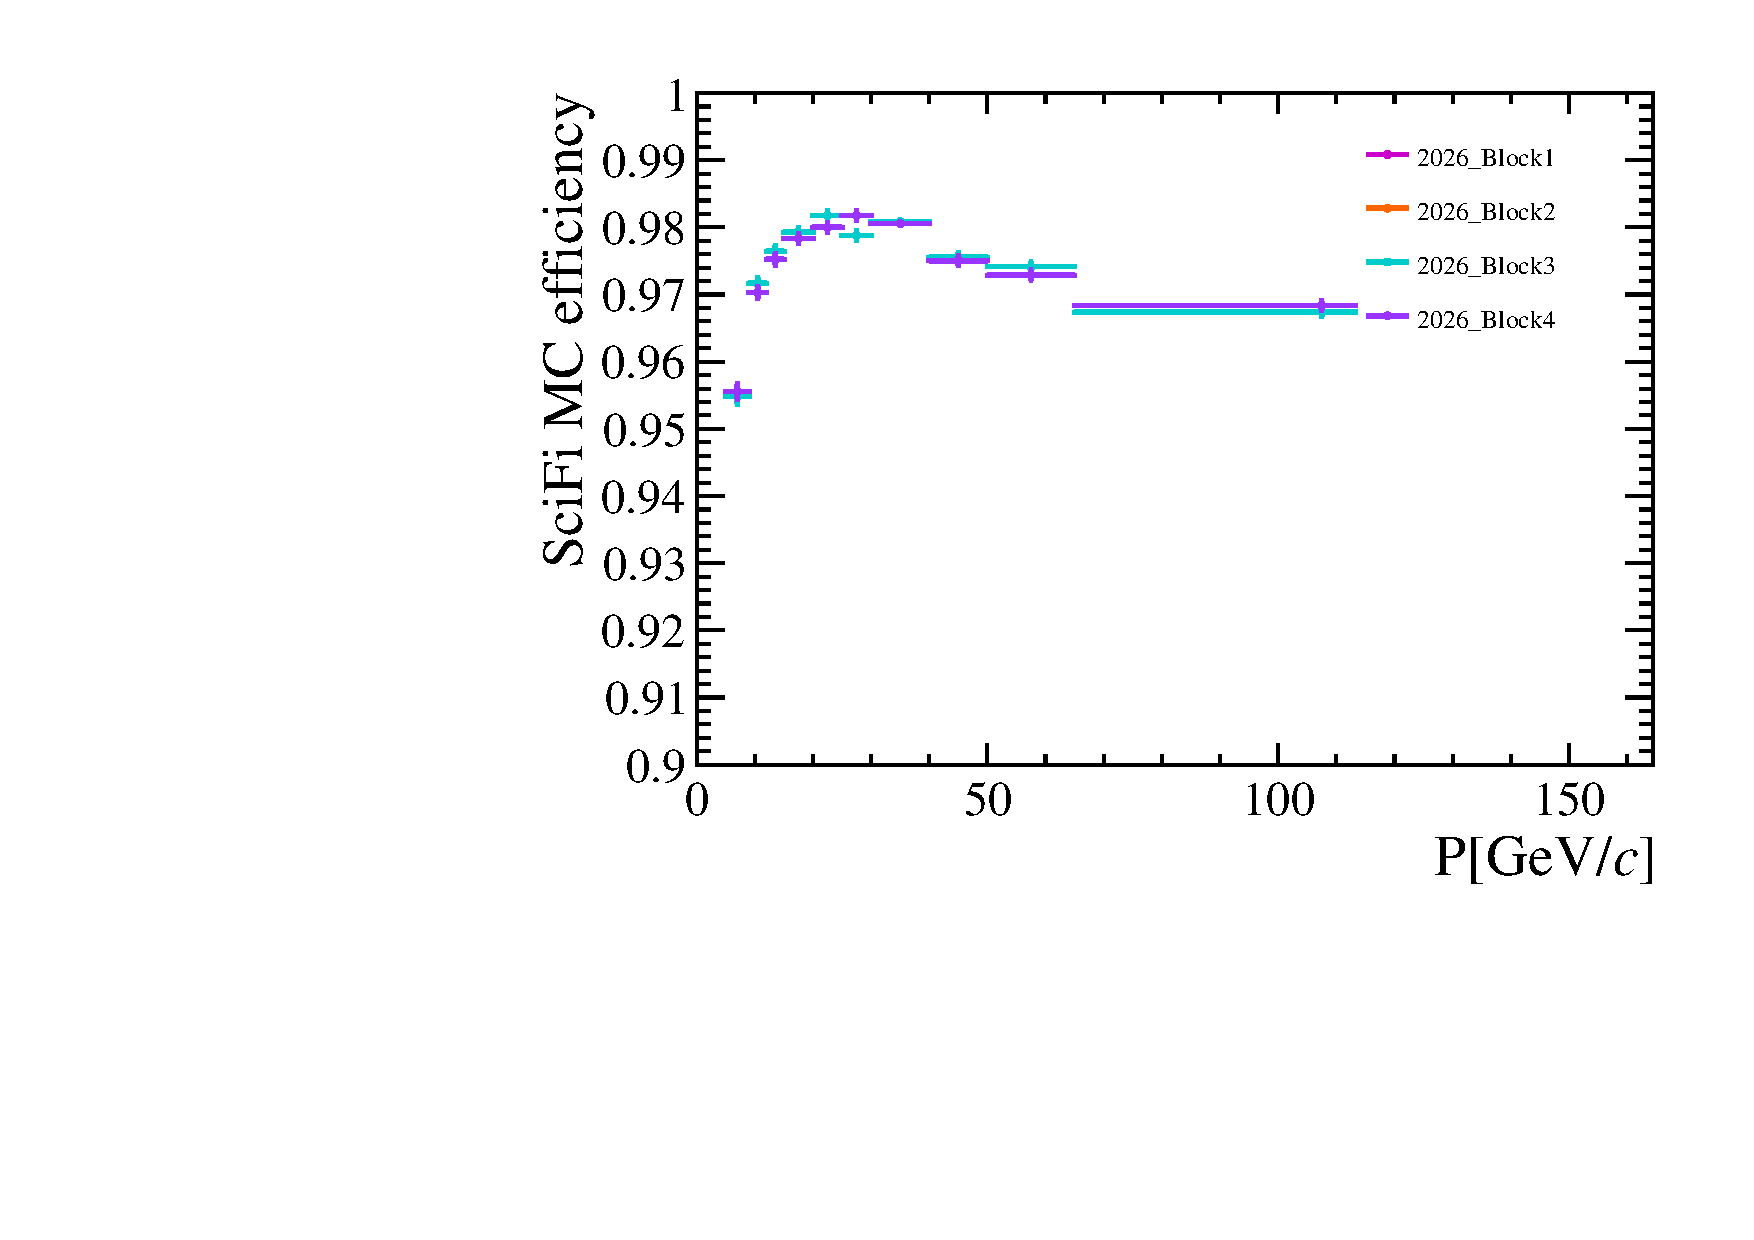
\includegraphics[width=1.0\textwidth]{Plots/trackeff_MC_VeloMuon_P_2026_expected_MC_samples.pdf}
    \end{subfigure}
  \end{figure}
  {SciFi efficiencies looks quite different between data and MC...}
\end{frame}

\begin{frame}{2026 tracking efficiencies}
  \vspace{0.0cm}
  {\large Comparison of tracking efficiencies in 2026 data blocks}
  \begin{figure}[htb]
    \centering
    \begin{subfigure}{0.5\textwidth}
      \centering
      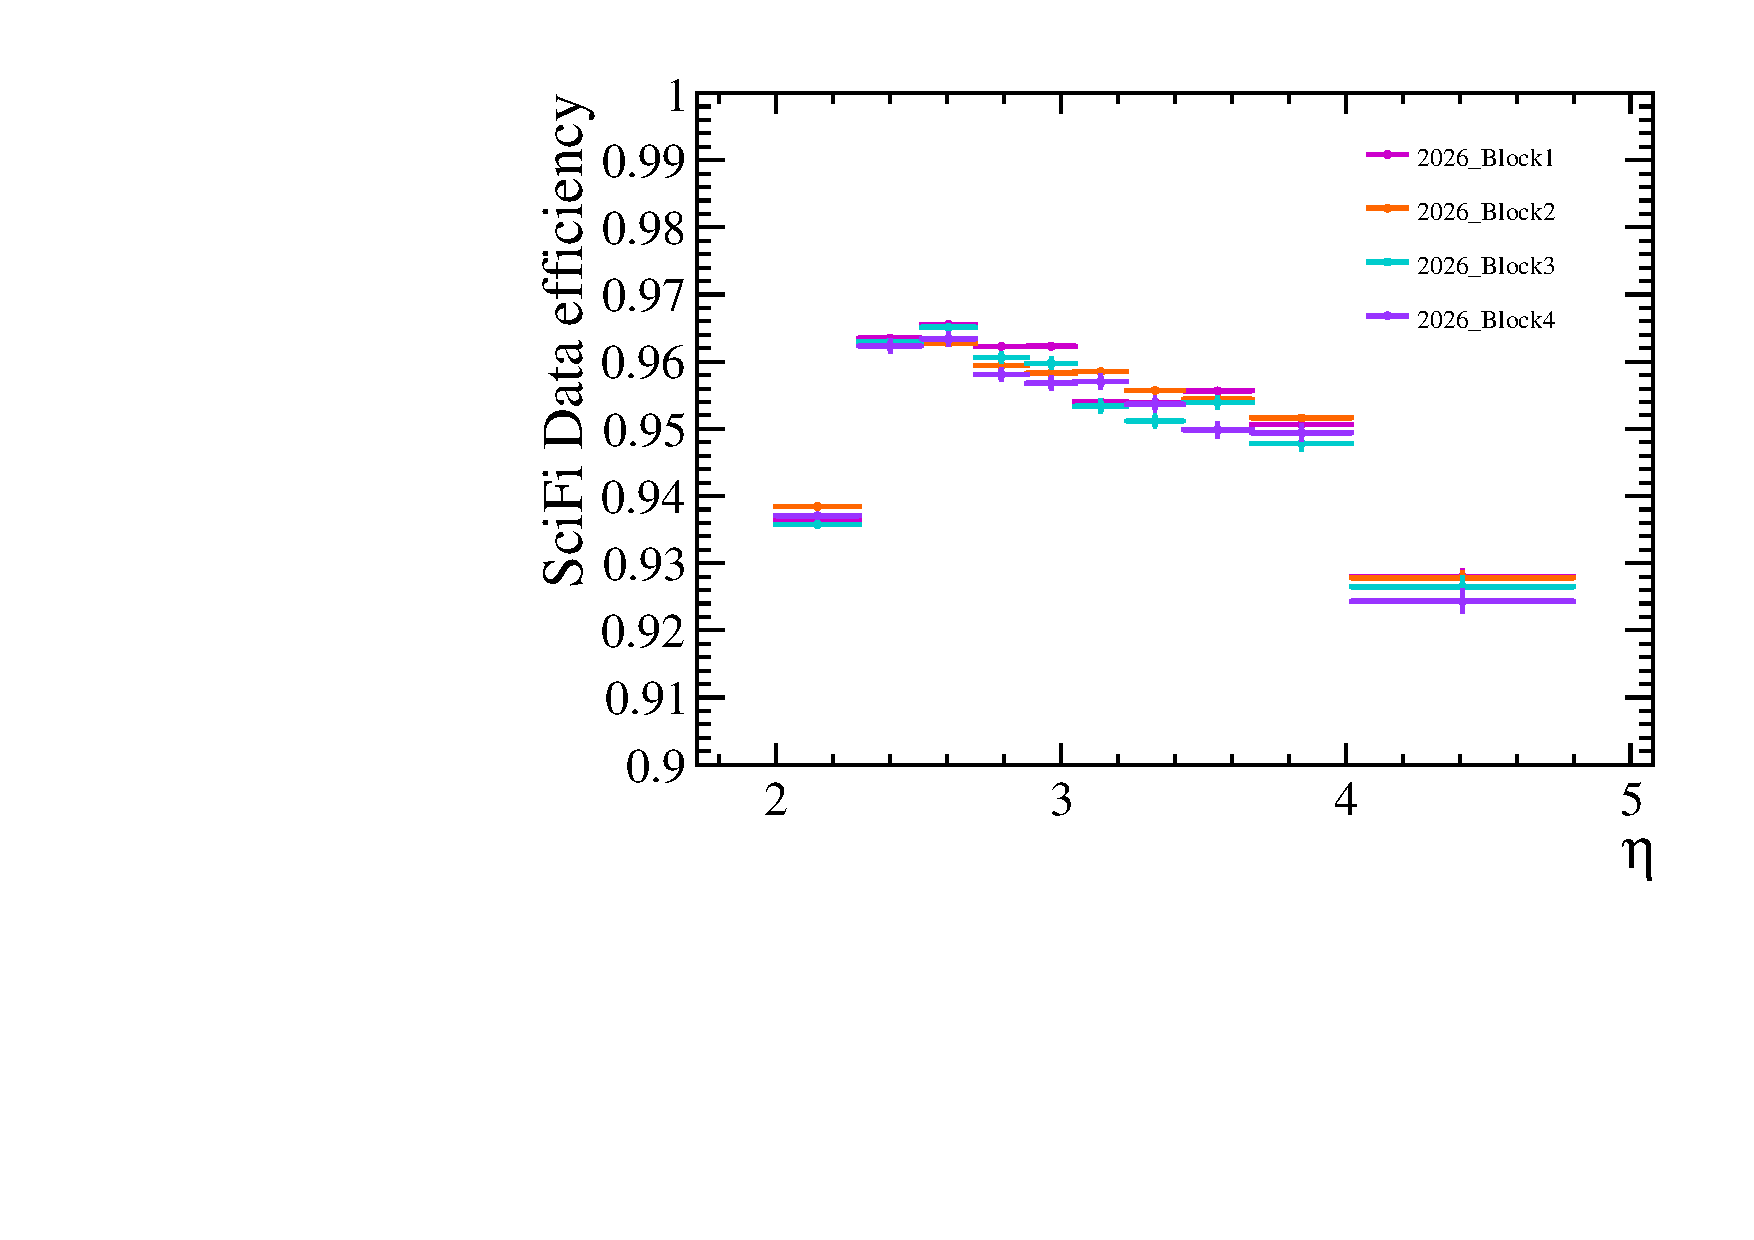
\includegraphics[width=1.0\textwidth]{Plots/trackeff_Data_VeloMuon_ETA_2026_expected_MC_samples.pdf}
    \end{subfigure}%
    \begin{subfigure}{0.5\textwidth}
      \centering
      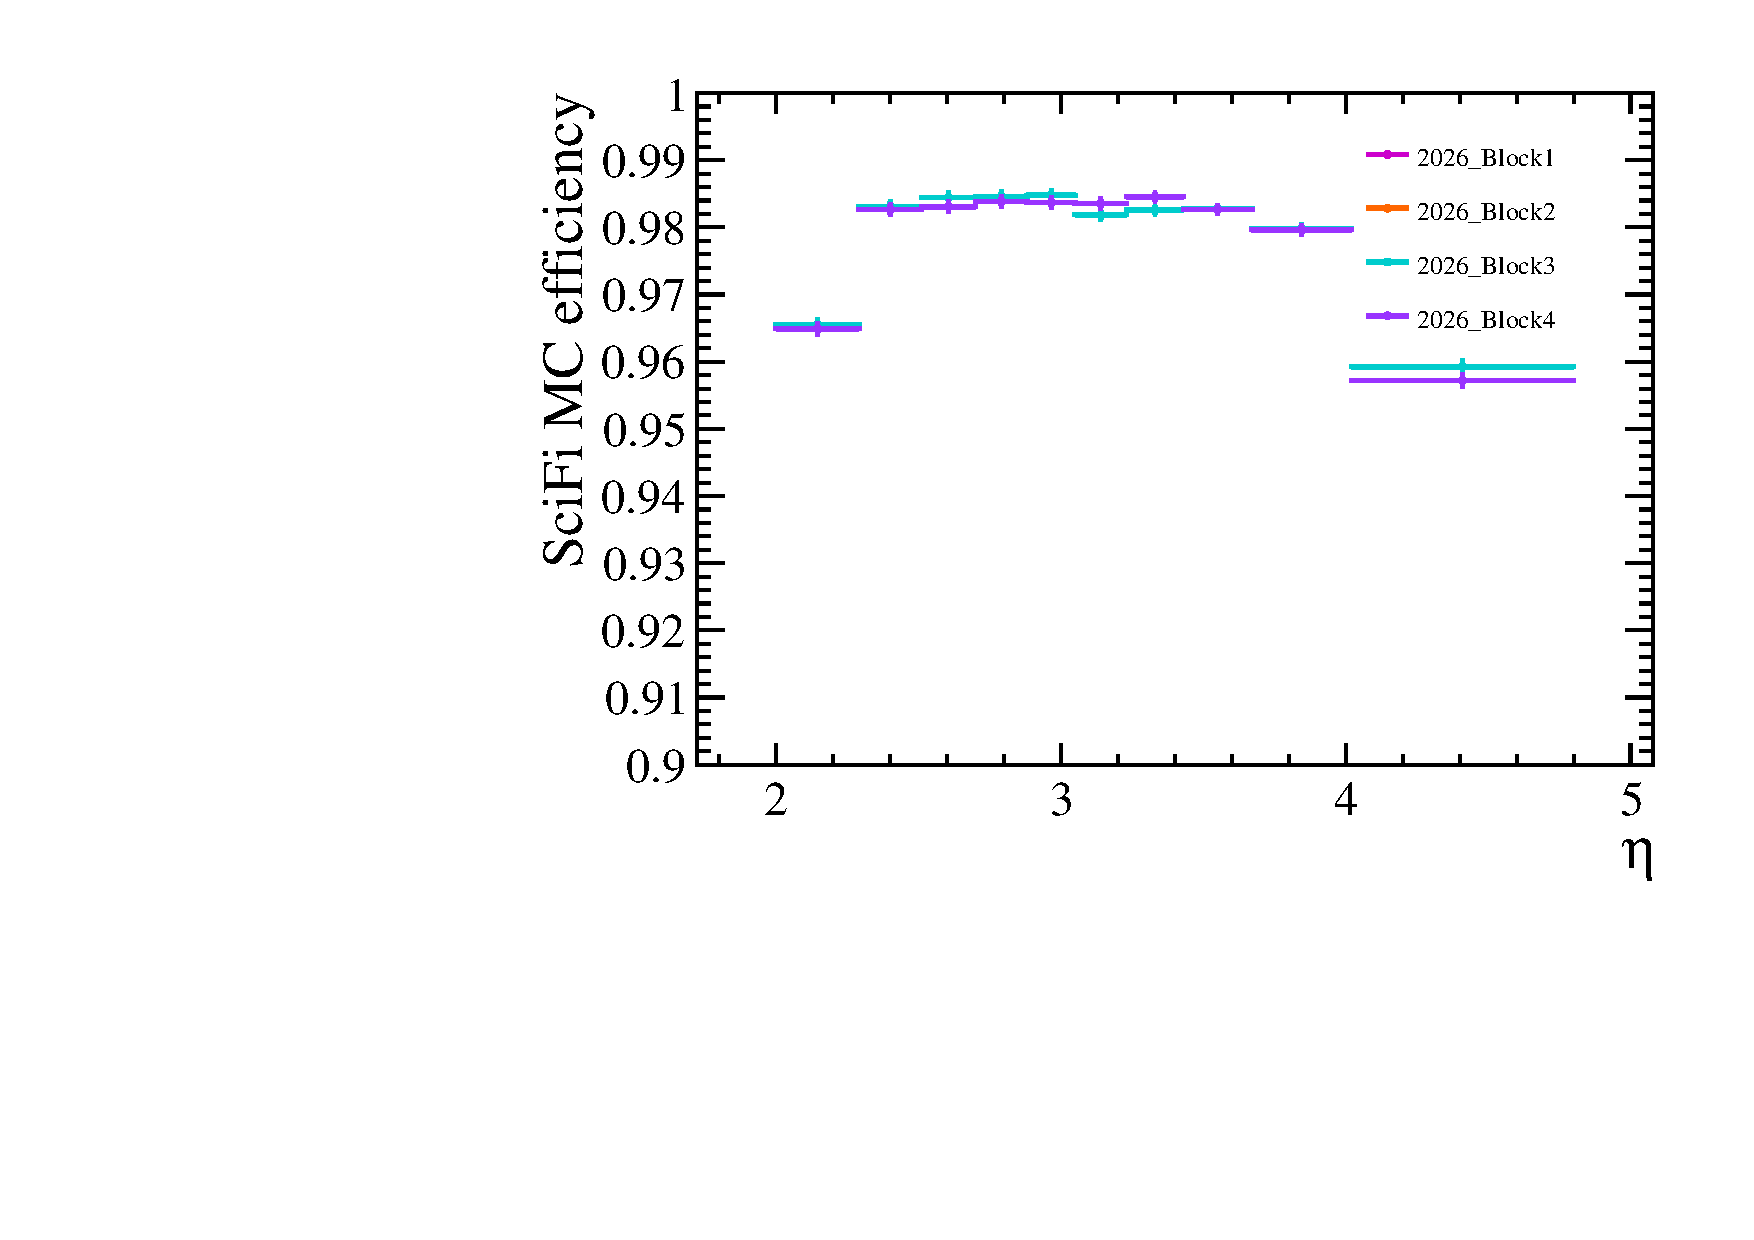
\includegraphics[width=1.0\textwidth]{Plots/trackeff_MC_VeloMuon_ETA_2026_expected_MC_samples.pdf}
    \end{subfigure}
  \end{figure}
  {SciFi efficiencies looks quite different between data and MC...}
\end{frame}

\begin{frame}{SciFi radiation damage?}
  \vspace{0.0cm}
  {\large Plot from RTA WP4/5 meeting on 4th June 2026:}
  \begin{figure}[htb]
    \centering
    \begin{subfigure}{0.5\textwidth}
      \centering
      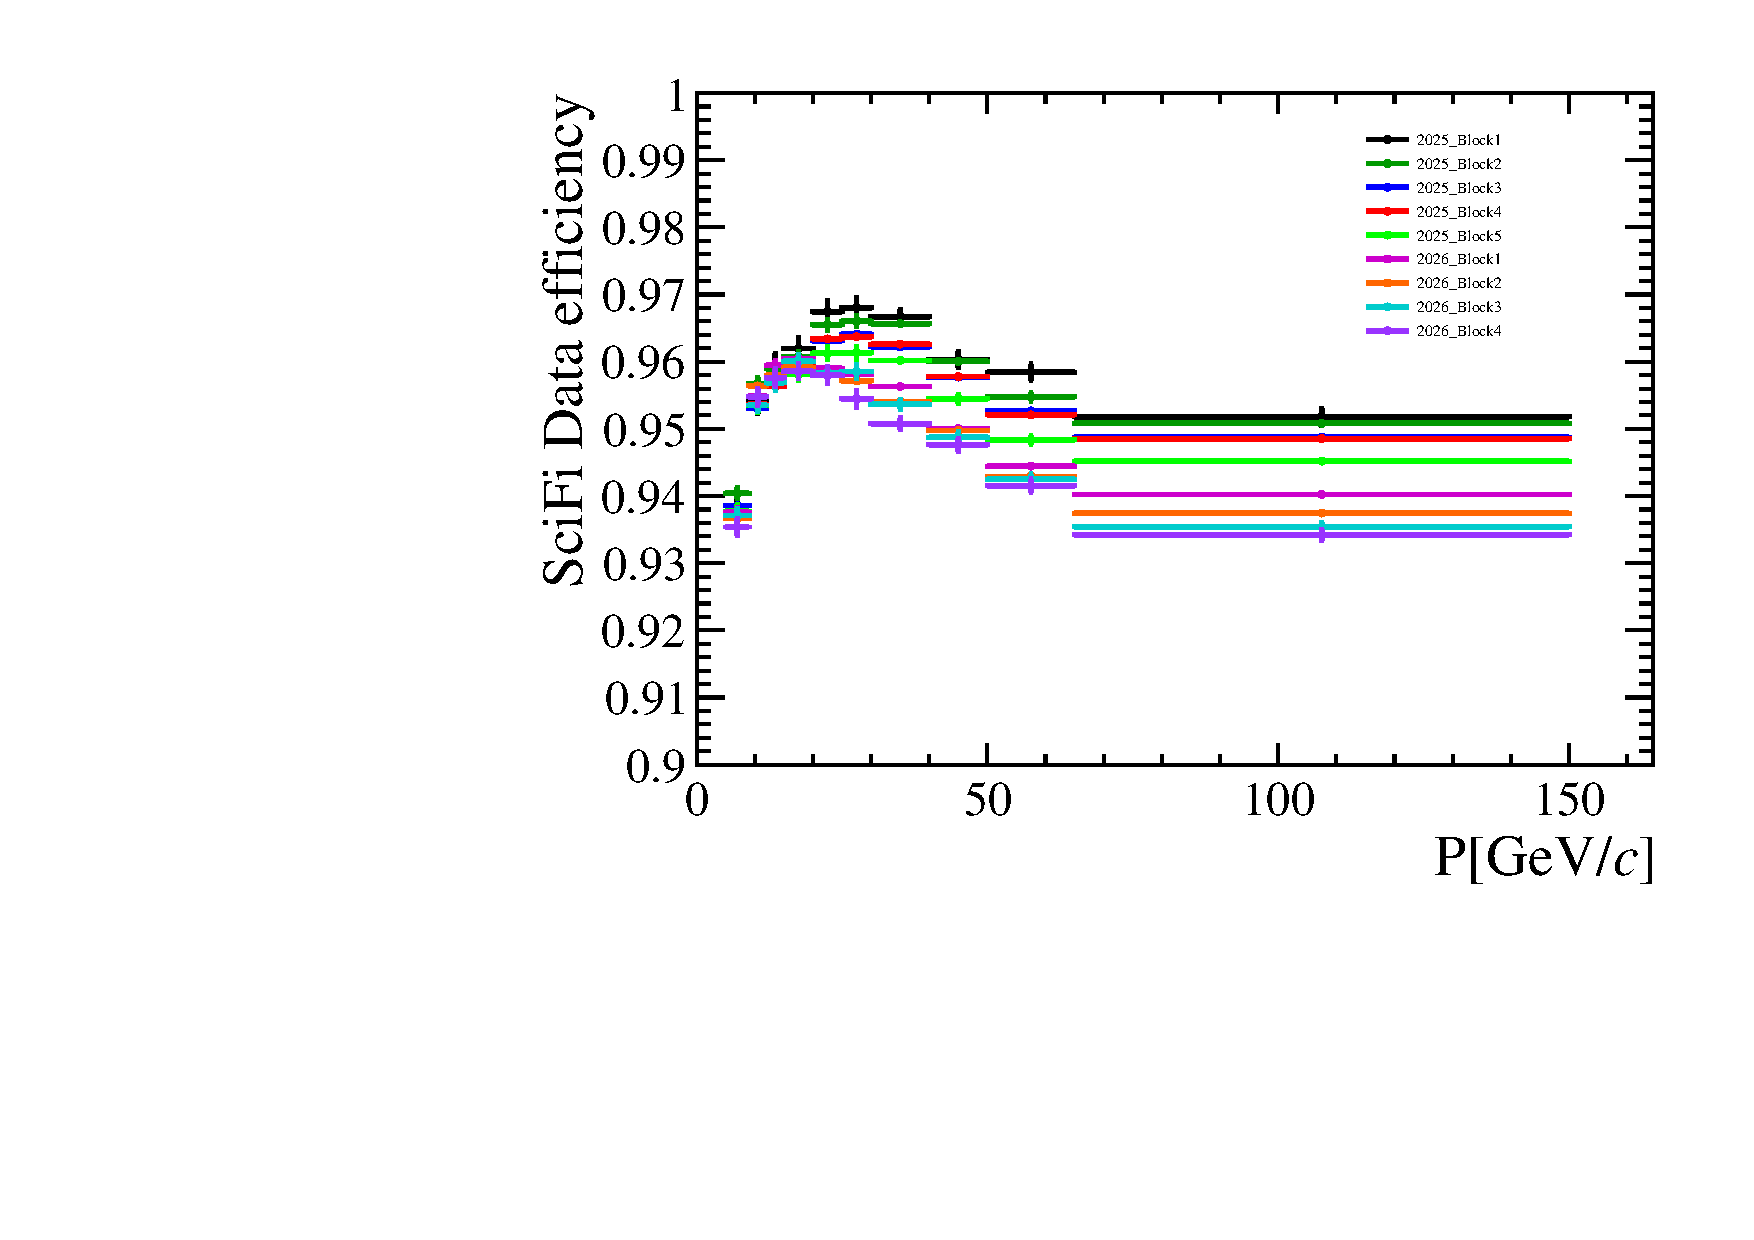
\includegraphics[width=1.0\textwidth]{Plots/trackeff_Data_VeloMuon_P_workdir_samples.pdf}
    \end{subfigure}%
    \begin{subfigure}{0.5\textwidth}
      \centering
      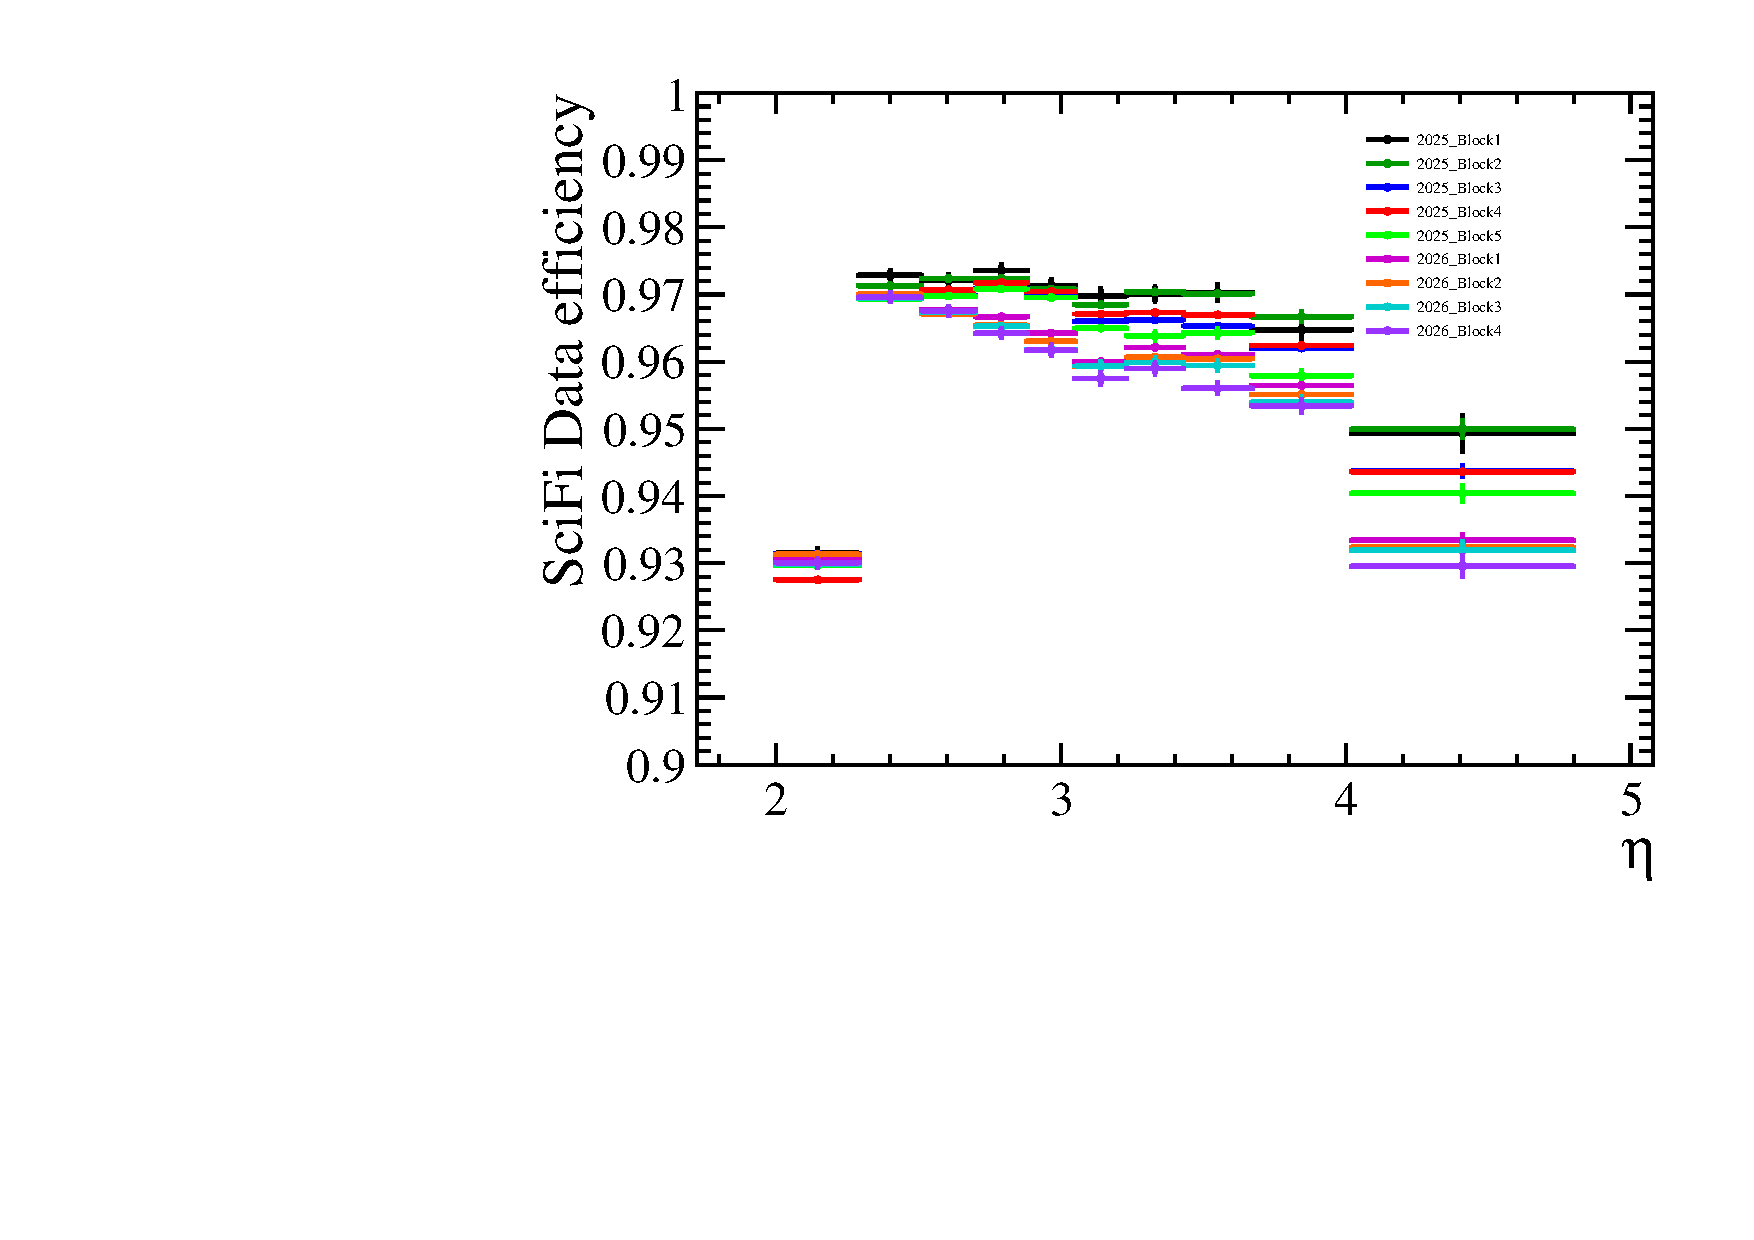
\includegraphics[width=1.0\textwidth]{Plots/trackeff_Data_VeloMuon_ETA_workdir_samples.pdf}
    \end{subfigure}
  \end{figure}
  \begin{itemize}
    \item{Clear signs of radiation damage at higher $\eta$...}
    \item{... but it is unclear what caused the drop between 2025 and 2026}
  \end{itemize}
\end{frame}

\begin{frame}{2026 tracking efficiencies}
  \vspace{0.0cm}
  {\large Comparison of tracking efficiencies in 2026 data blocks}
  \begin{figure}[htb]
    \centering
    \begin{subfigure}{0.5\textwidth}
      \centering
      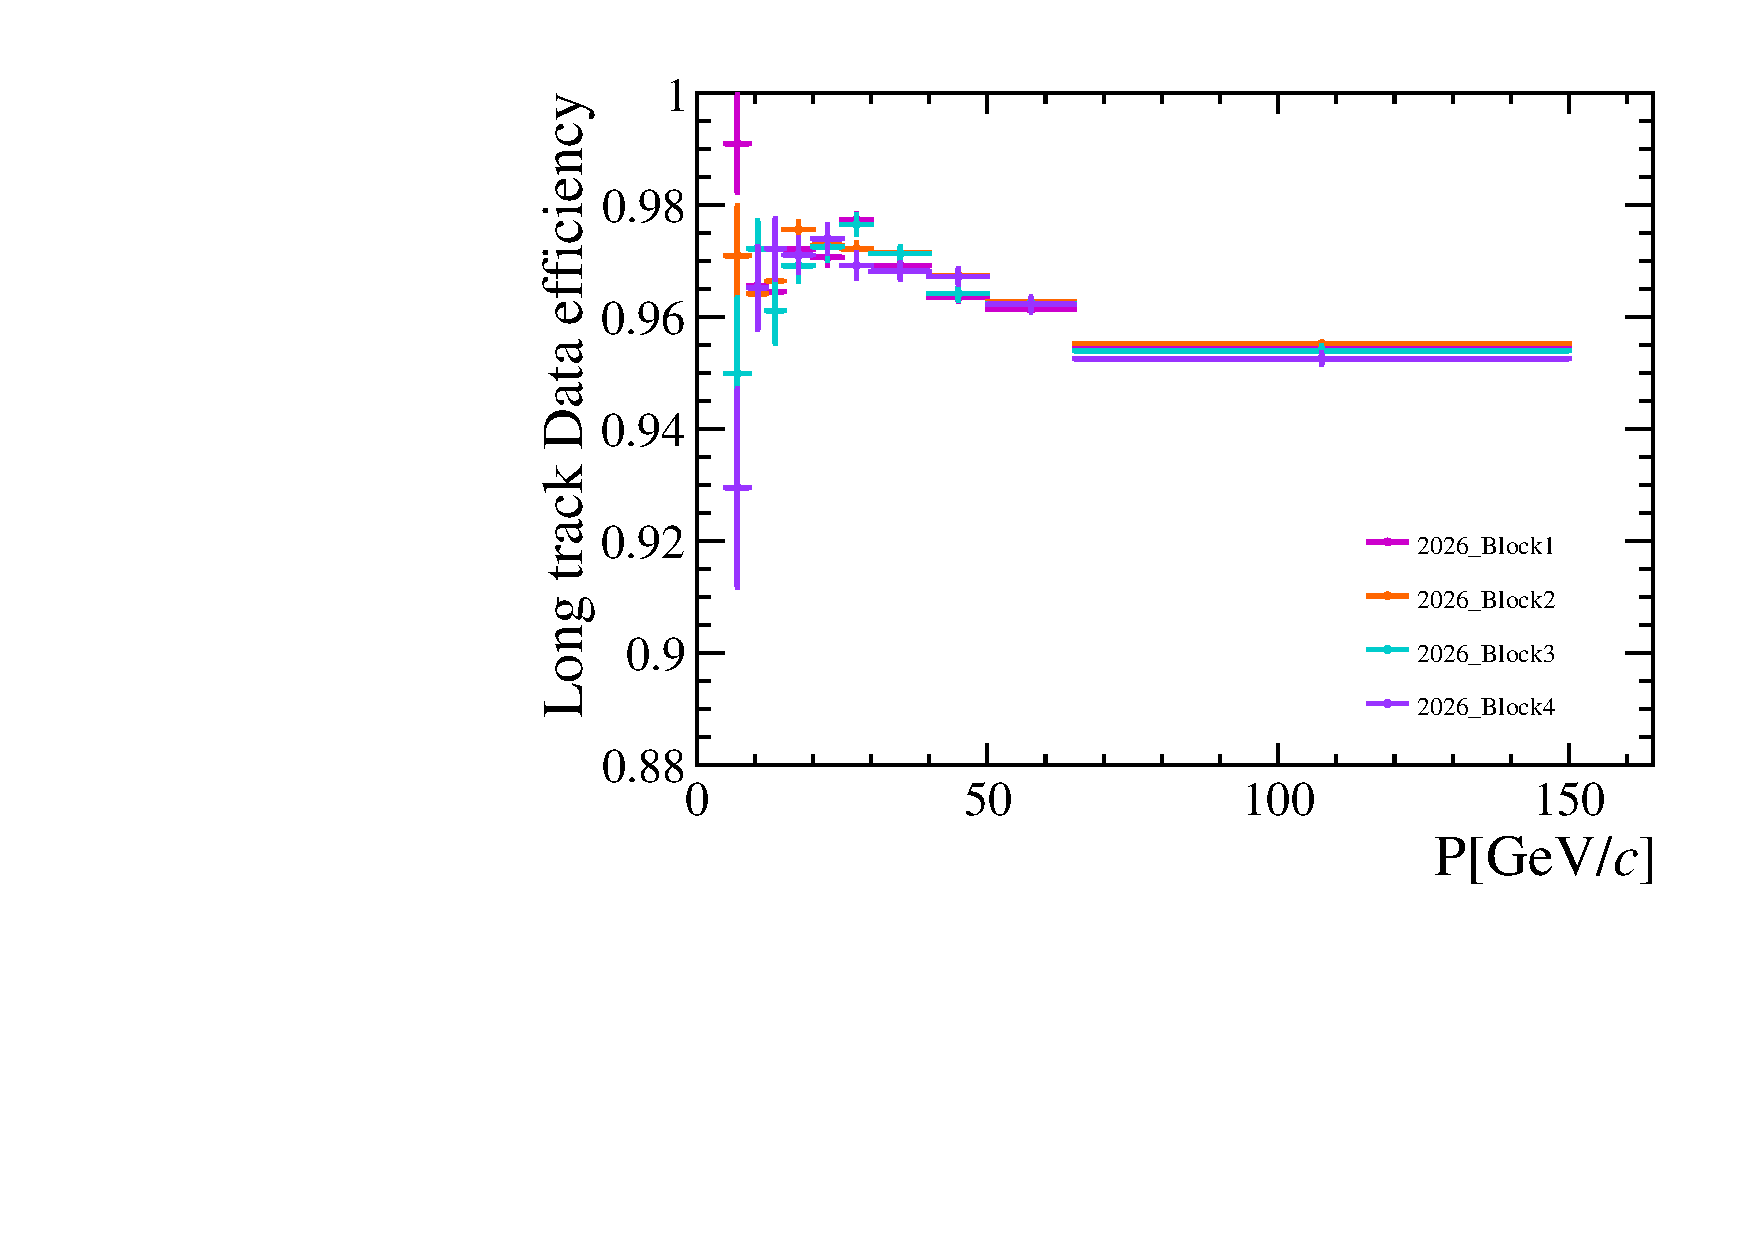
\includegraphics[width=1.0\textwidth]{Plots/trackeff_Data_MuonUT_P_2026_expected_MC_samples.pdf}
    \end{subfigure}%
    \begin{subfigure}{0.5\textwidth}
      \centering
      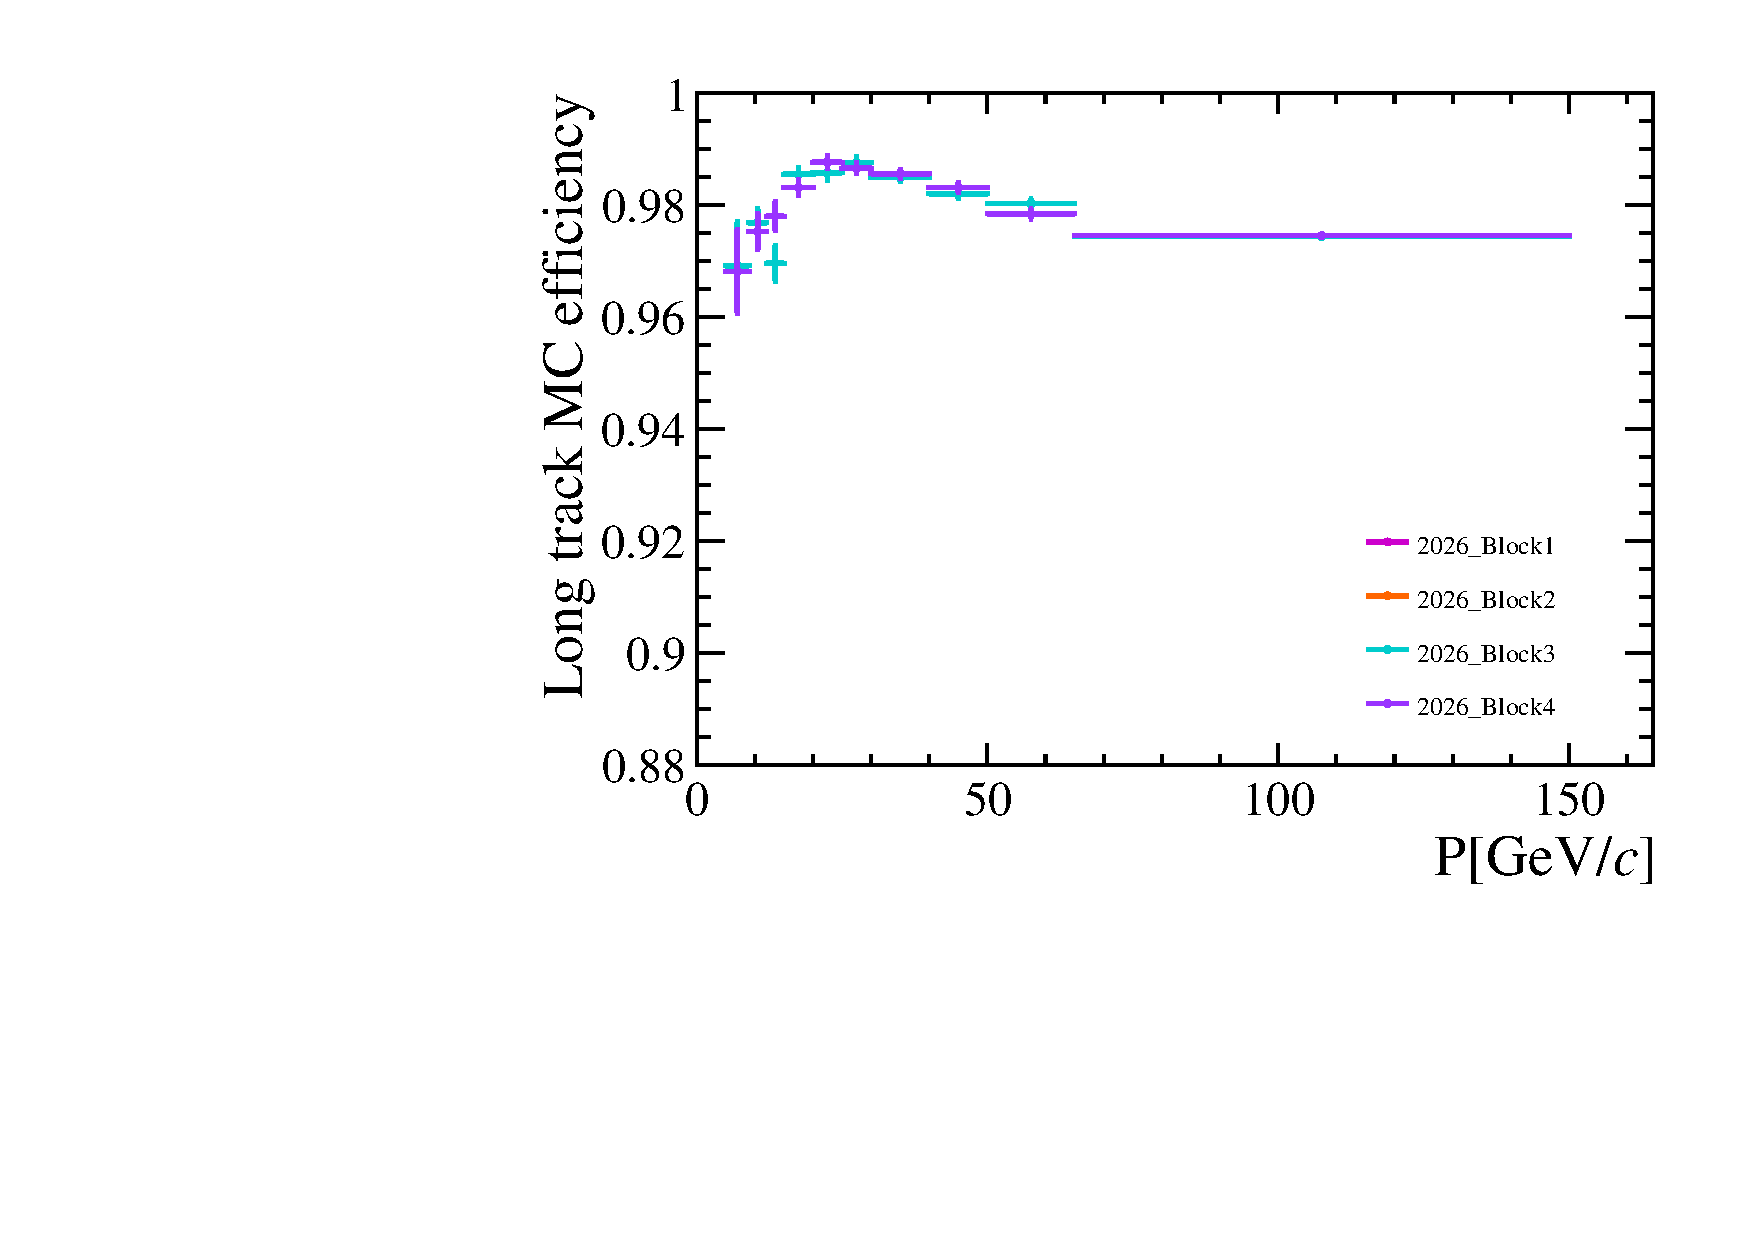
\includegraphics[width=1.0\textwidth]{Plots/trackeff_MC_MuonUT_P_2026_expected_MC_samples.pdf}
    \end{subfigure}
  \end{figure}
  {MuonUT efficiencies have consistent trend between data and MC}
\end{frame}

\begin{frame}{2026 tracking efficiencies}
  \vspace{0.0cm}
  {\large Comparison of tracking efficiencies in 2026 data blocks}
  \begin{figure}[htb]
    \centering
    \begin{subfigure}{0.5\textwidth}
      \centering
      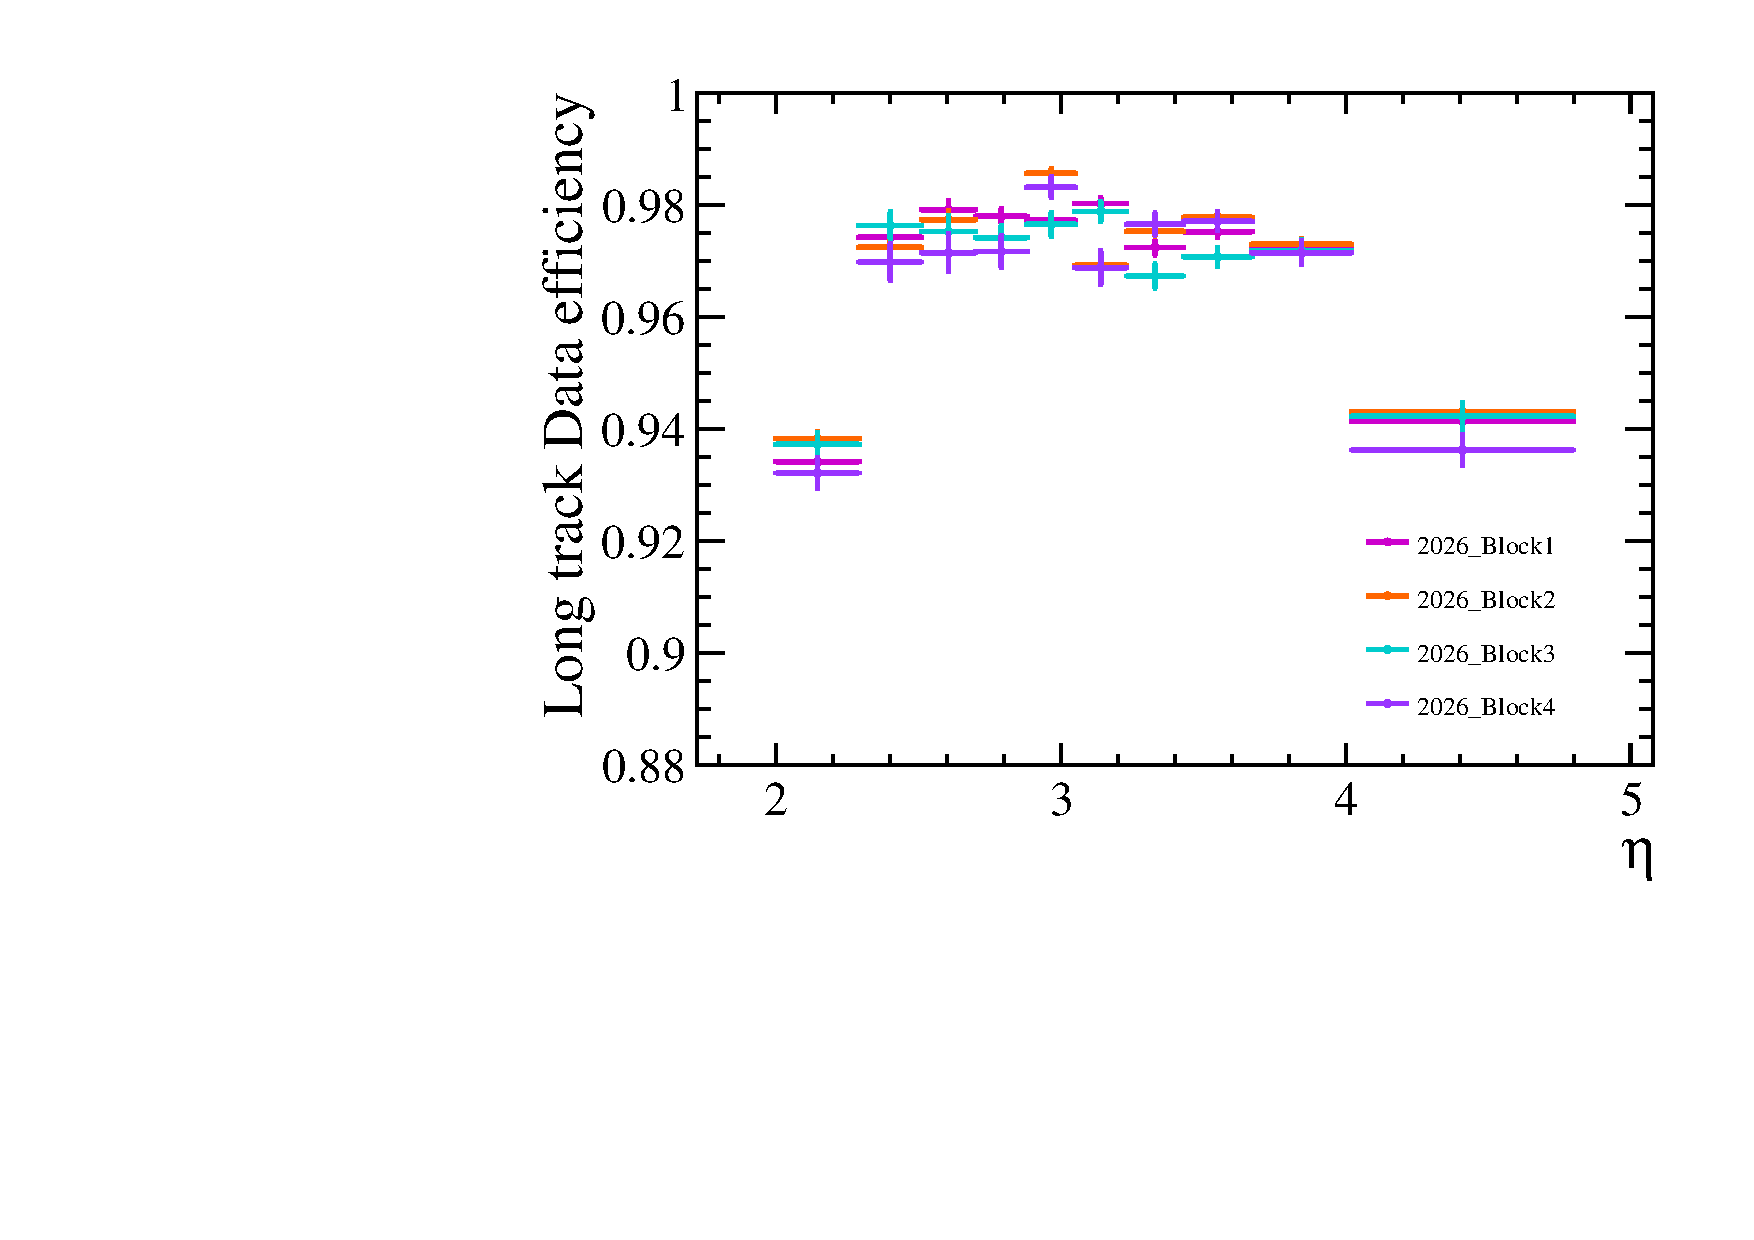
\includegraphics[width=1.0\textwidth]{Plots/trackeff_Data_MuonUT_ETA_2026_expected_MC_samples.pdf}
    \end{subfigure}%
    \begin{subfigure}{0.5\textwidth}
      \centering
      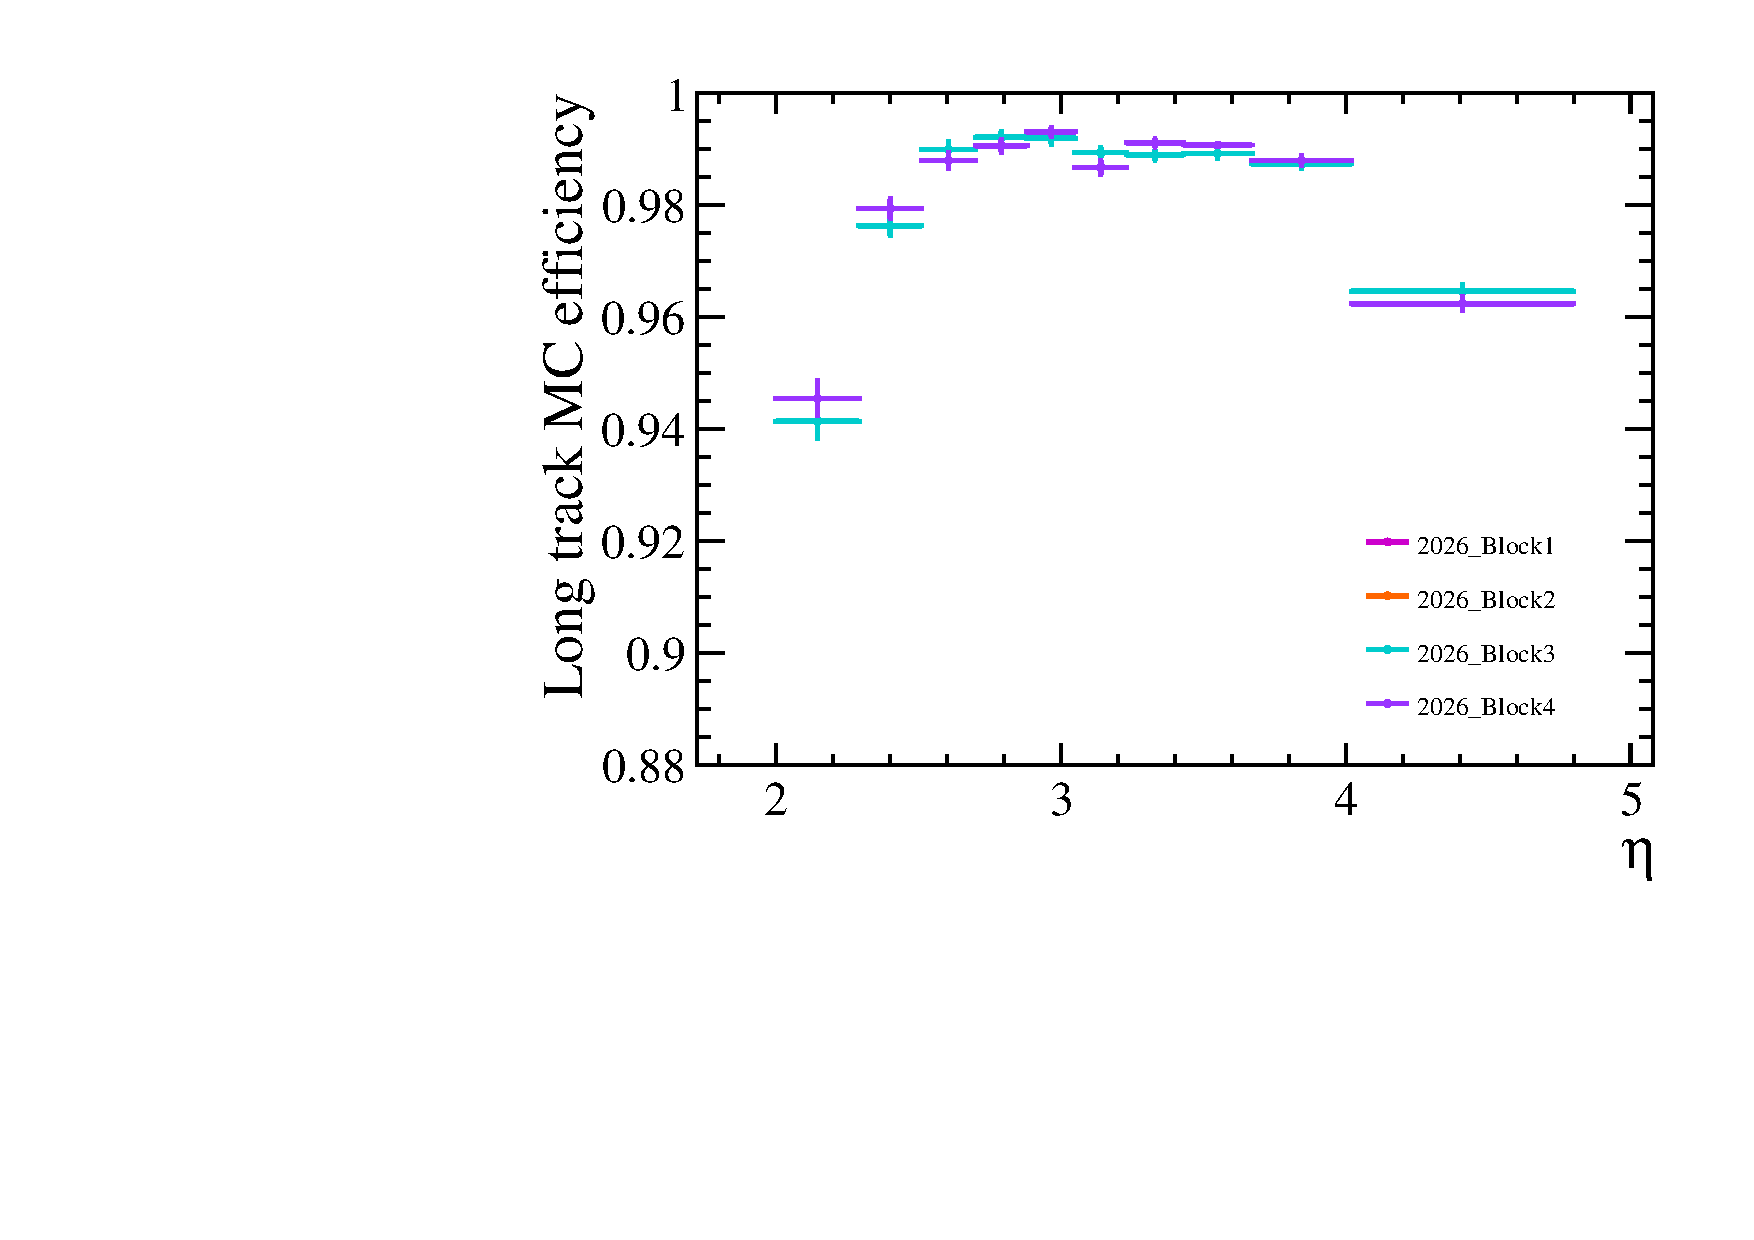
\includegraphics[width=1.0\textwidth]{Plots/trackeff_MC_MuonUT_ETA_2026_expected_MC_samples.pdf}
    \end{subfigure}
  \end{figure}
  {MuonUT efficiencies have consistent trend between data and MC}
\end{frame}

\begin{frame}{2026 tracking efficiency ratios}
  \vspace{0.0cm}
  {\large Comparison of tracking efficiency ratios in 2026 Block 1}
  \begin{figure}[htb]
    \centering
    \begin{subfigure}{0.5\textwidth}
      \centering
      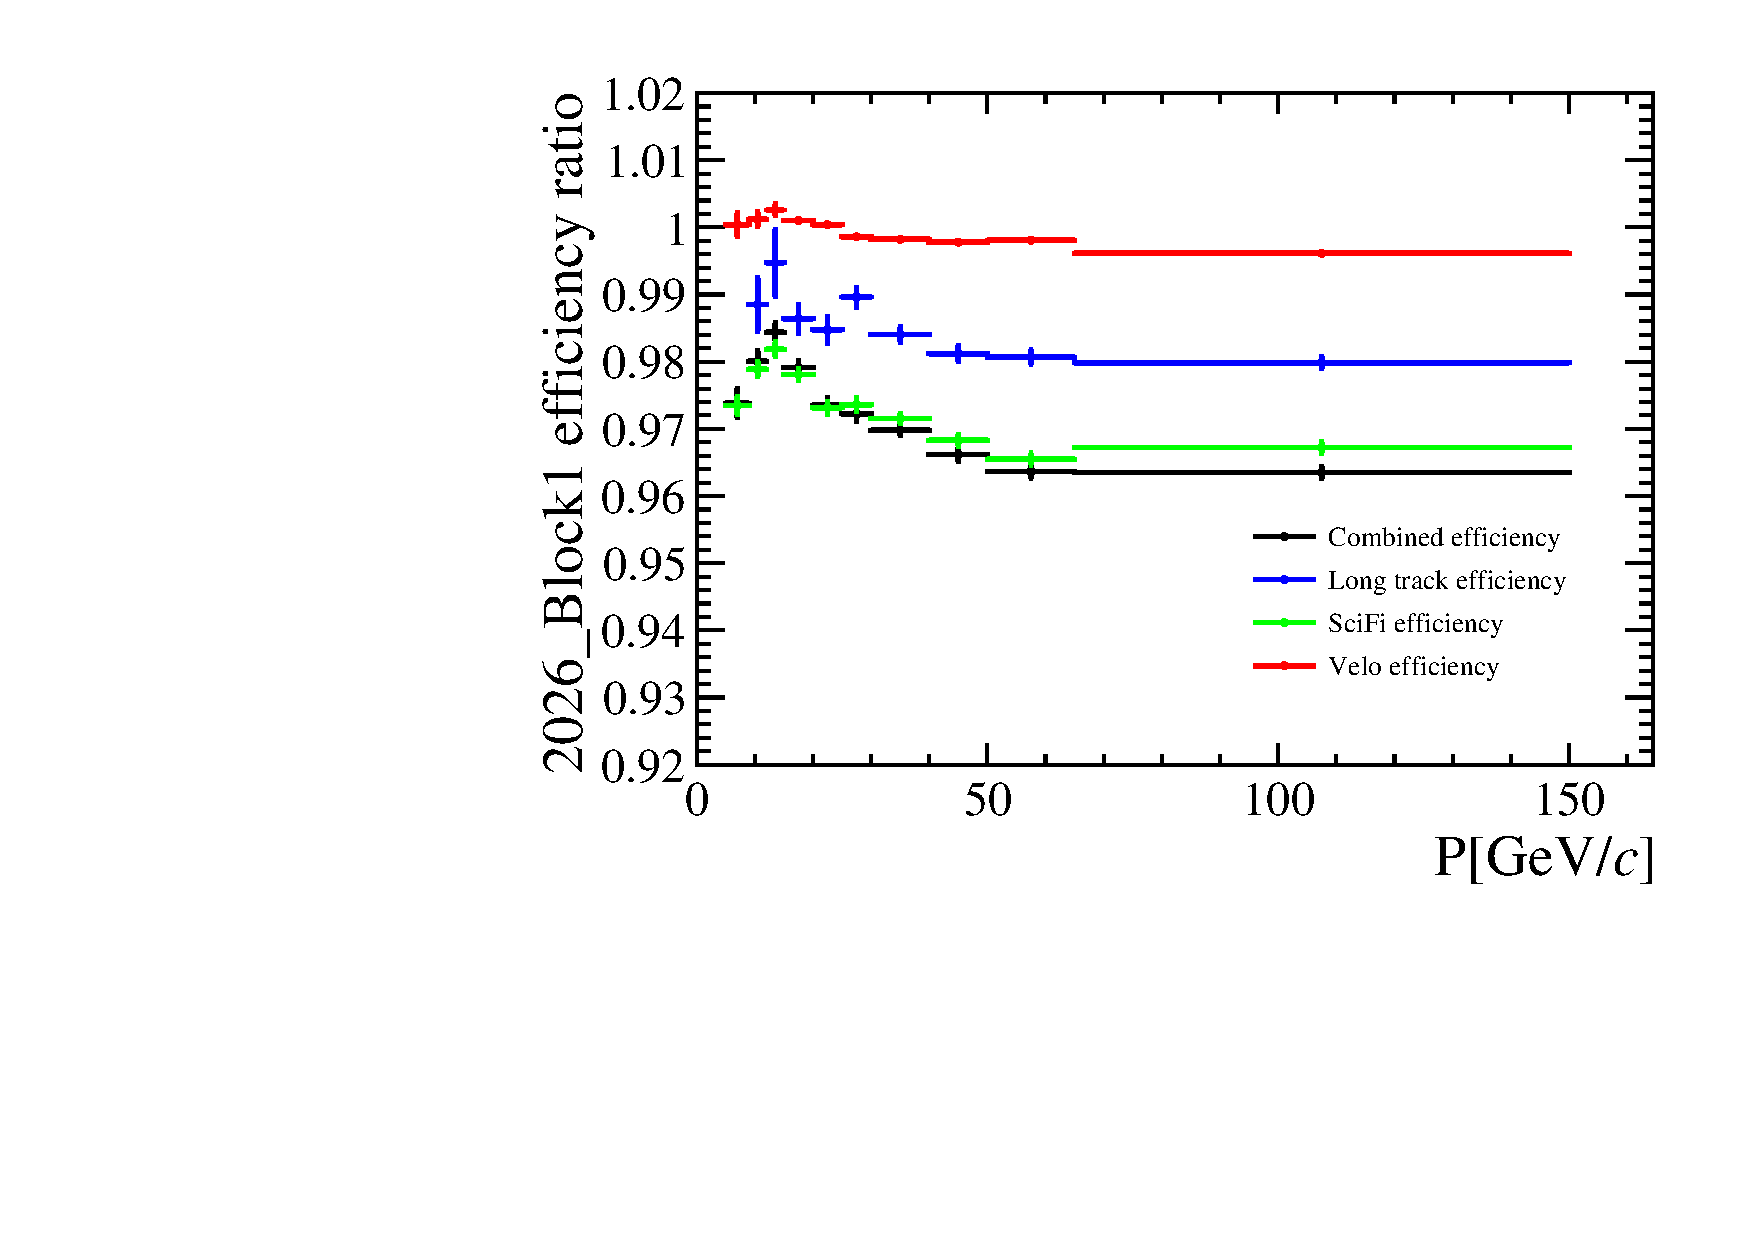
\includegraphics[width=1.0\textwidth]{Plots/trackeff_ratio_P_2026_Block1_2026_expected_MC_samples.pdf}
    \end{subfigure}%
    \begin{subfigure}{0.5\textwidth}
      \centering
      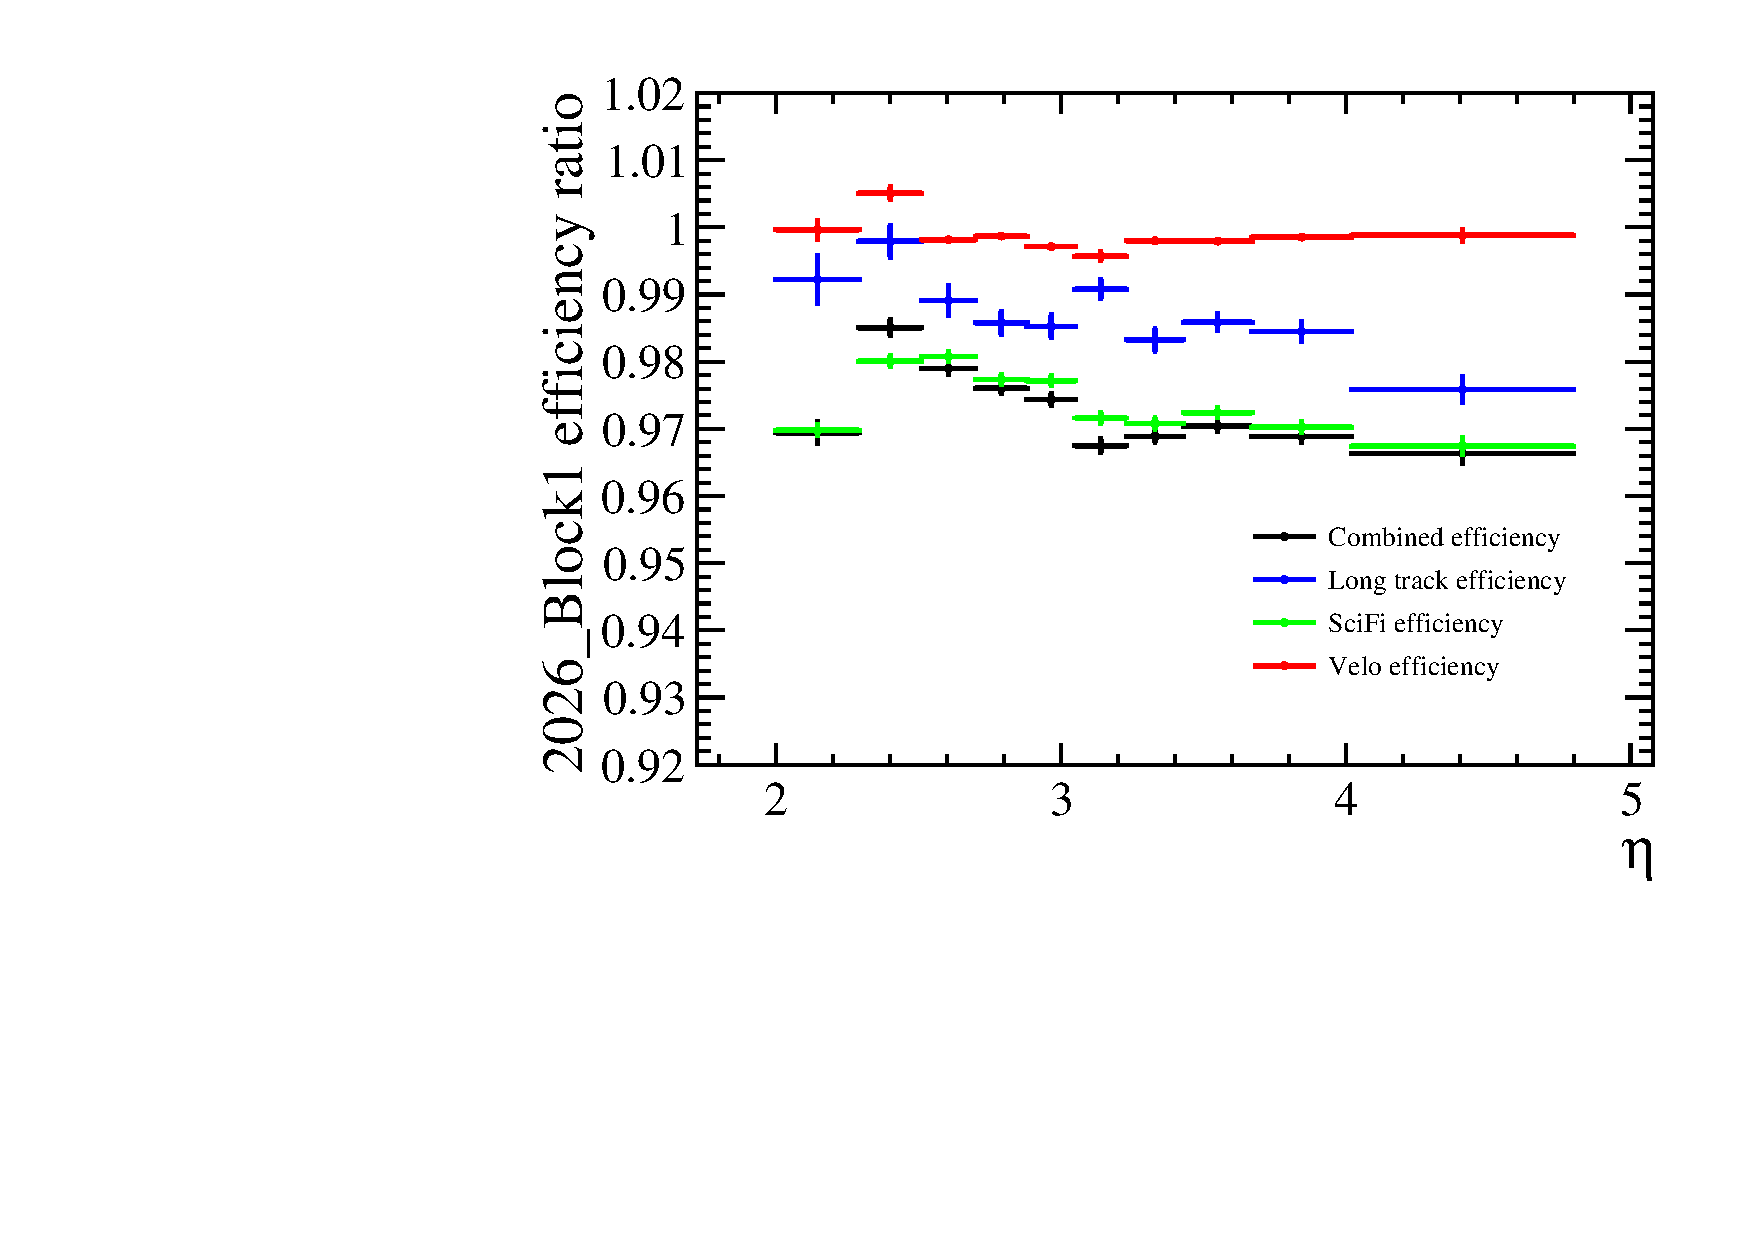
\includegraphics[width=1.0\textwidth]{Plots/trackeff_ratio_ETA_2026_Block1_2026_expected_MC_samples.pdf}
    \end{subfigure}
  \end{figure}
  {No surprises in 2026 Block 1}
\end{frame}

\begin{frame}{2026 tracking efficiency ratios}
  \vspace{0.0cm}
  {\large Comparison of tracking efficiency ratios in 2026 Block 2}
  \begin{figure}[htb]
    \centering
    \begin{subfigure}{0.5\textwidth}
      \centering
      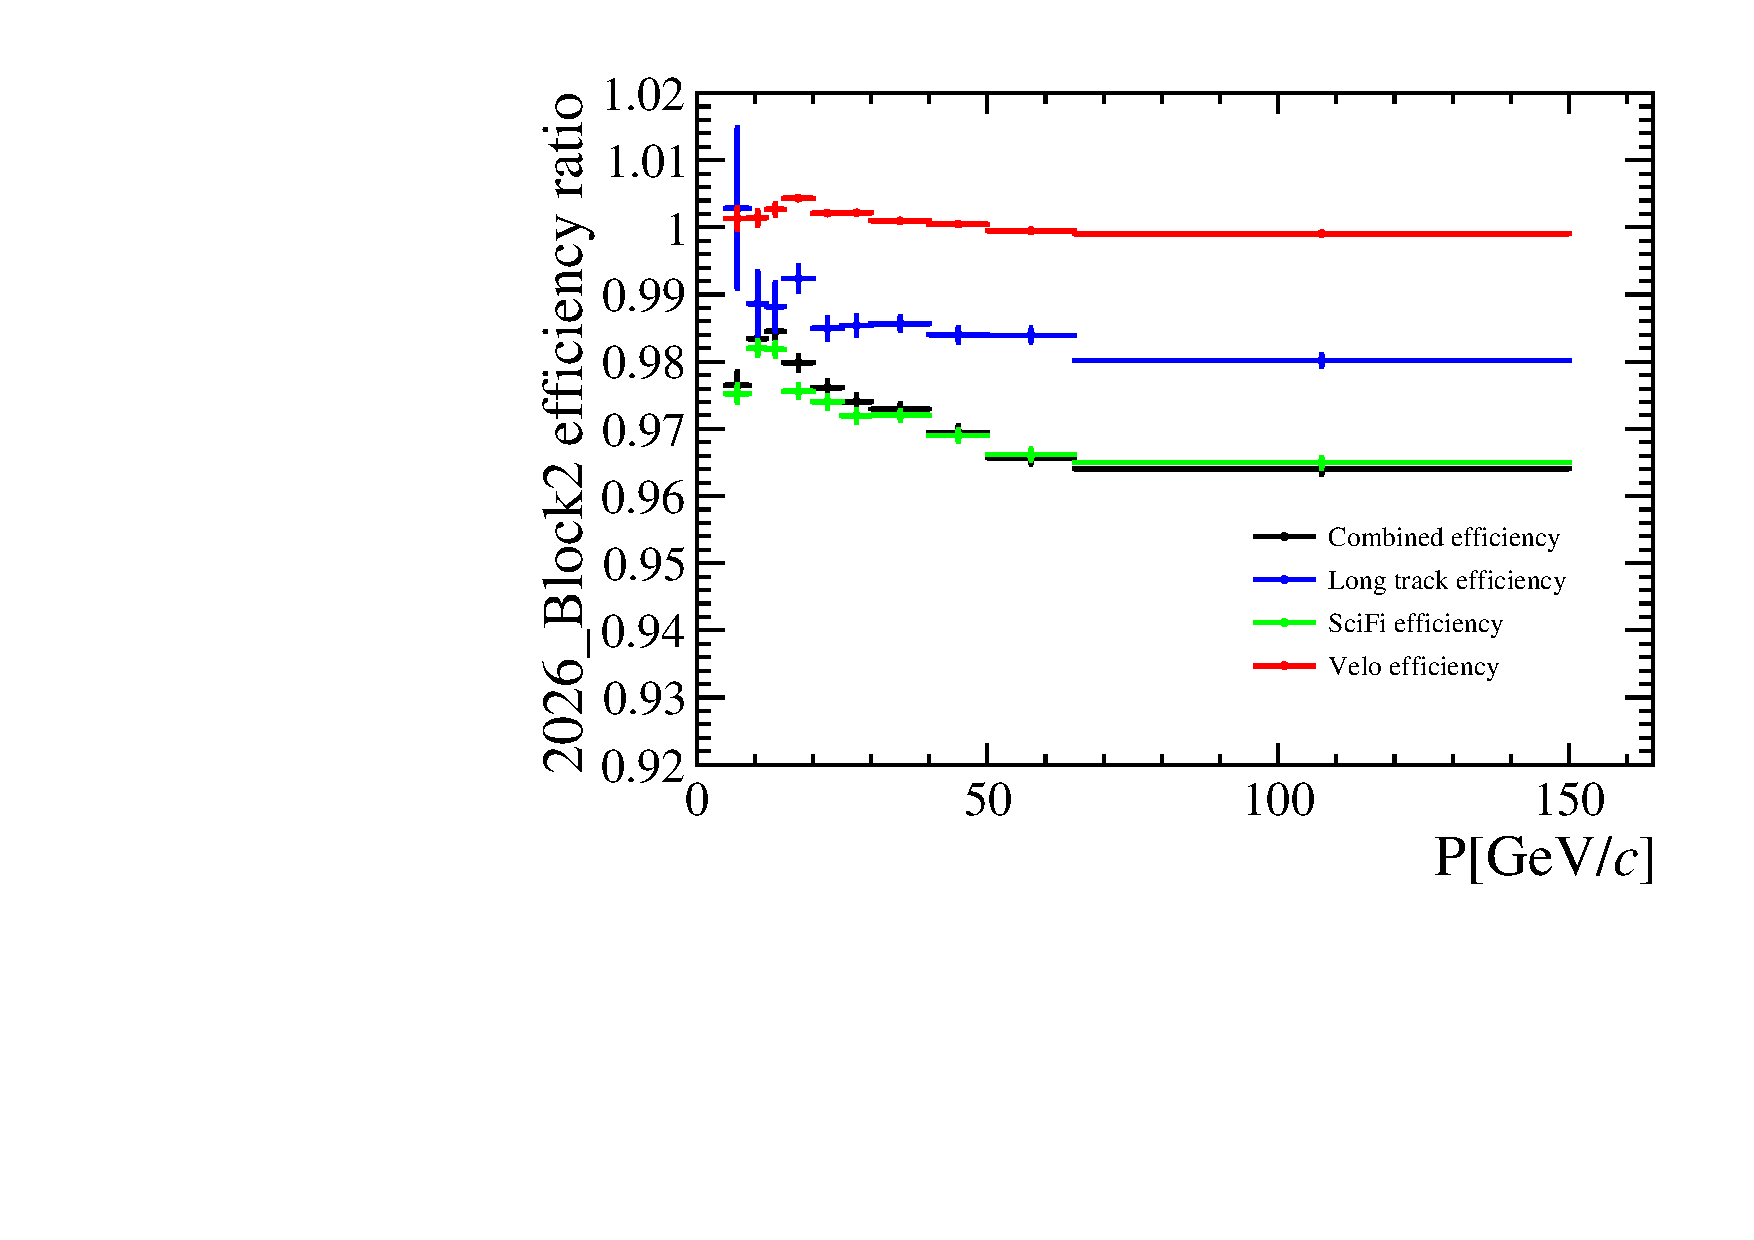
\includegraphics[width=1.0\textwidth]{Plots/trackeff_ratio_P_2026_Block2_2026_expected_MC_samples.pdf}
    \end{subfigure}%
    \begin{subfigure}{0.5\textwidth}
      \centering
      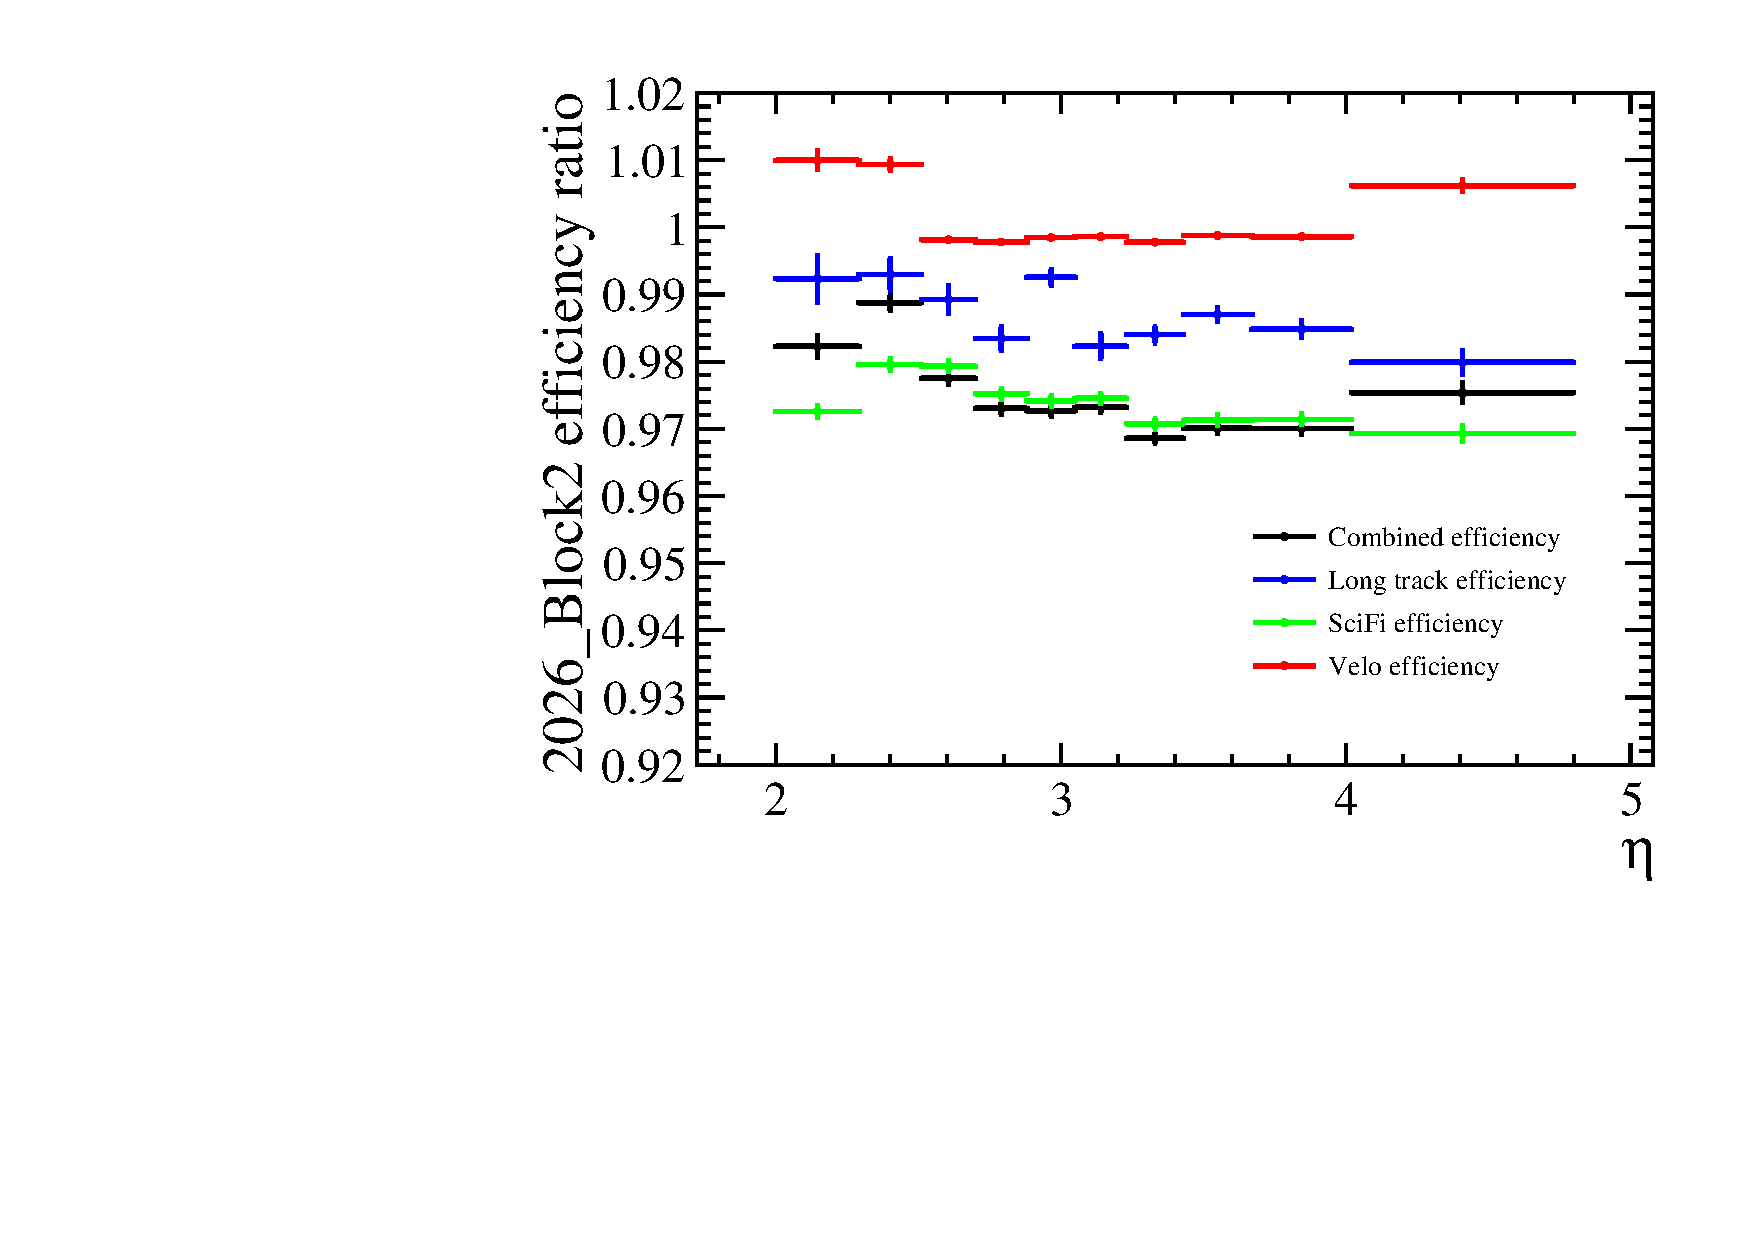
\includegraphics[width=1.0\textwidth]{Plots/trackeff_ratio_ETA_2026_Block2_2026_expected_MC_samples.pdf}
    \end{subfigure}
  \end{figure}
  {2026 Block 2 shows some discrepancies in Velo efficiencies}
\end{frame}

\begin{frame}{2D binning}
  \vspace{0.0cm}
  {\large 2D binning in $p$ vs $\eta$ with 72 bins:}
  \vspace{-0.3cm}
  \begin{figure}[htb]
    \centering
    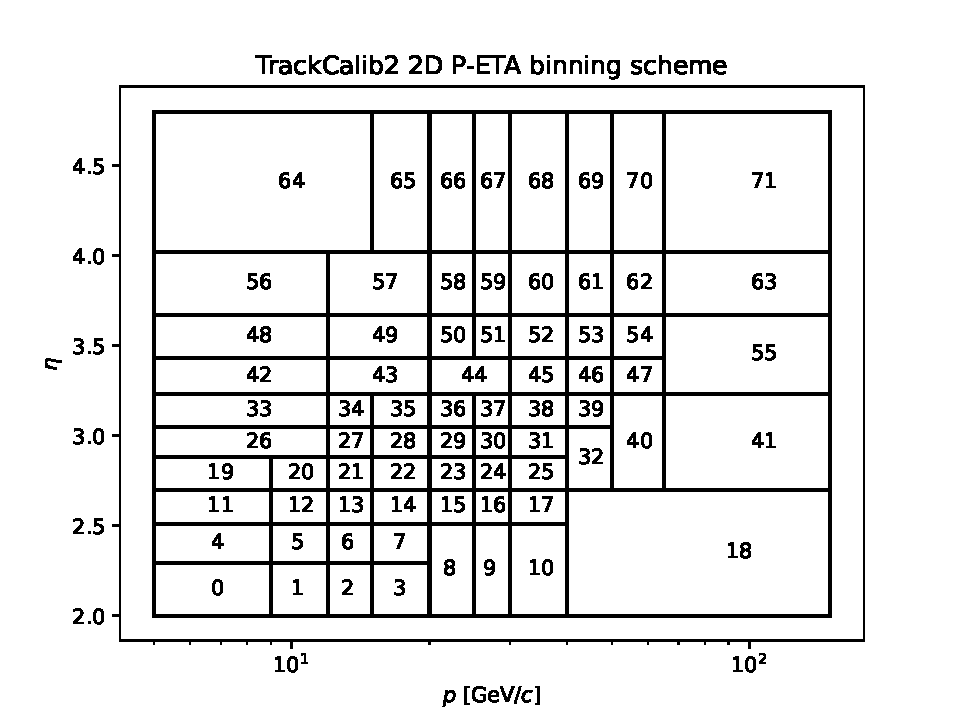
\includegraphics[width=0.8\textwidth]{Plots/TrackCalib2_2D_binning_scheme.pdf}
  \end{figure}
\end{frame}

\begin{frame}{2D binning}
  \vspace{0.0cm}
  \begin{figure}[htb]
    \centering
    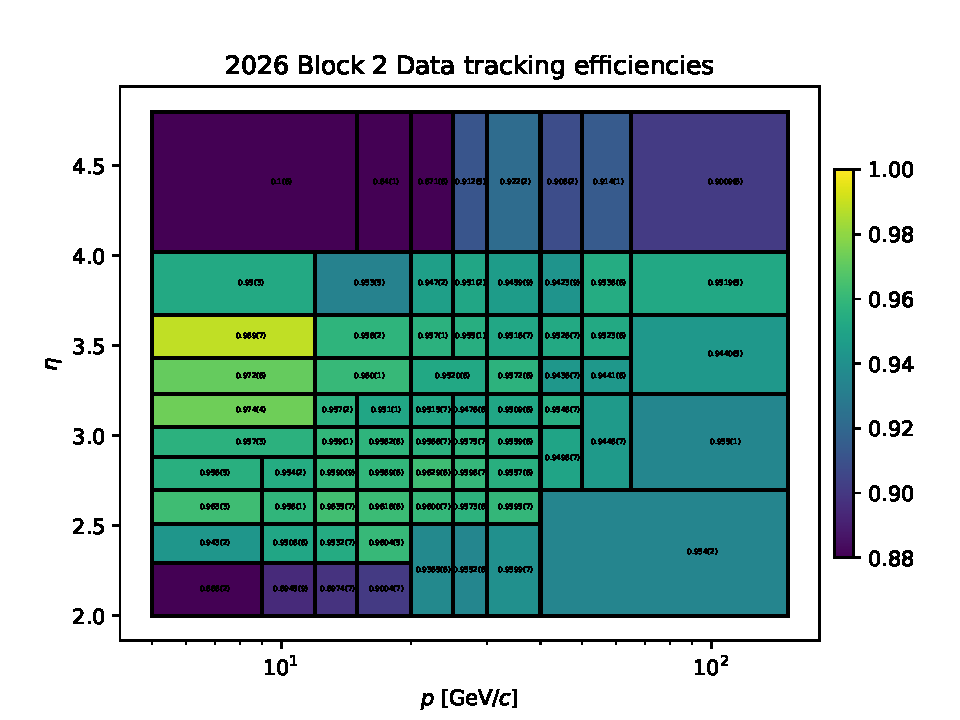
\includegraphics[width=0.85\textwidth]{Plots/TrackingEfficiencies_2D_binning_2026_Block2_Data_colour.pdf}
  \end{figure}
\end{frame}

\begin{frame}{2D binning}
  \vspace{0.0cm}
  \begin{figure}[htb]
    \centering
    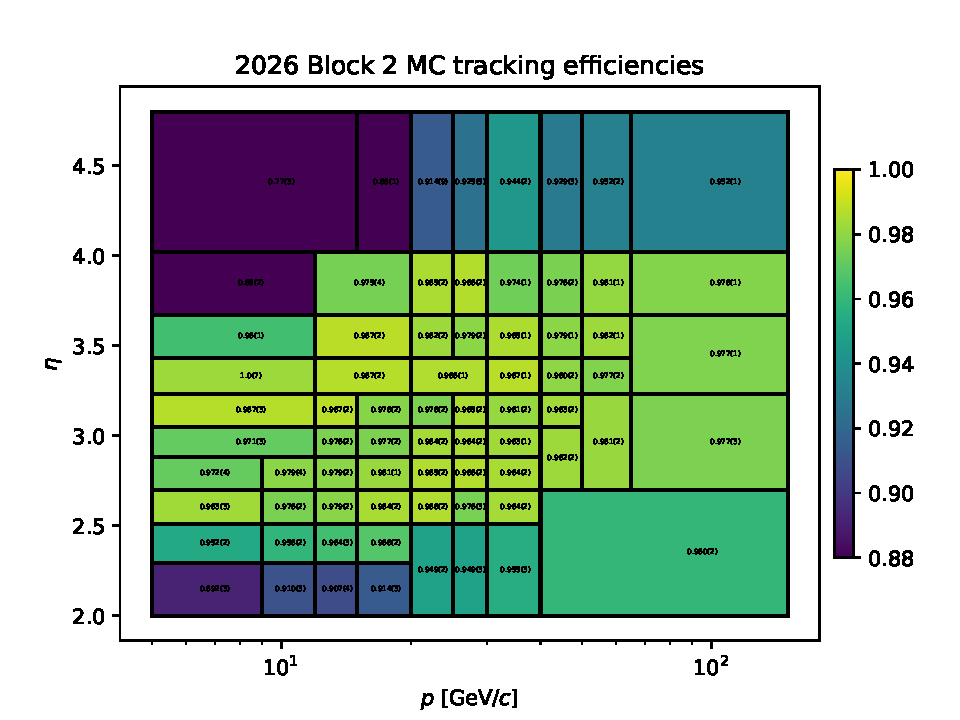
\includegraphics[width=0.85\textwidth]{Plots/TrackingEfficiencies_2D_binning_2026_Block2_MC_colour.pdf}
  \end{figure}
\end{frame}

\begin{frame}{2D binning}
  \vspace{0.0cm}
  \begin{figure}[htb]
    \centering
    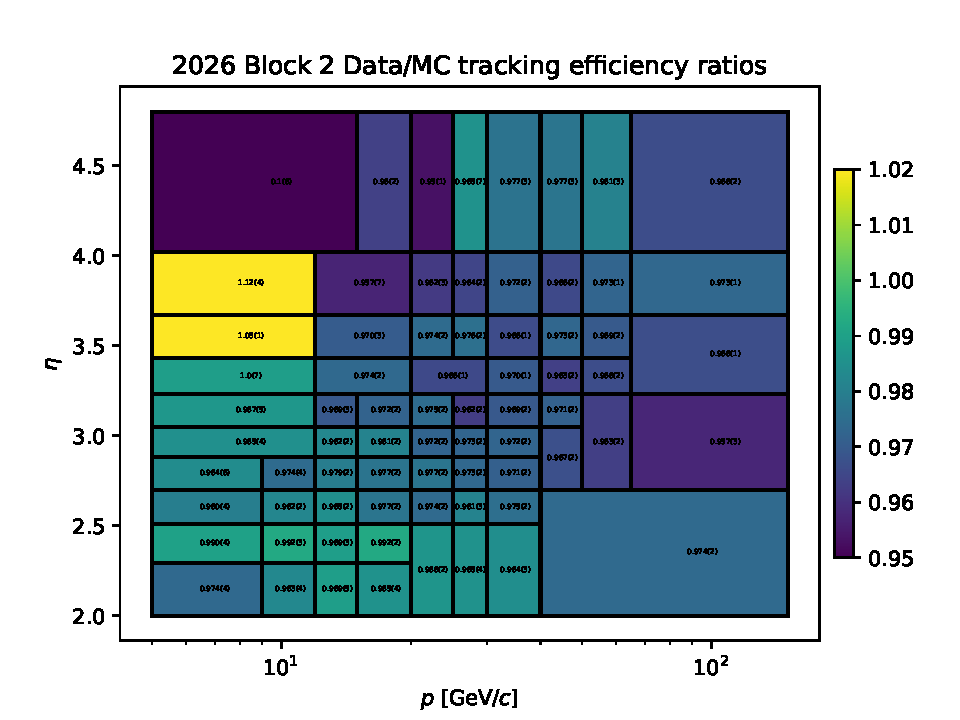
\includegraphics[width=0.85\textwidth]{Plots/TrackingEfficiencies_2D_binning_2026_Block2_Ratio_colour.pdf}
  \end{figure}
\end{frame}

\begin{frame}{2D binning}
  \vspace{0.0cm}
  \begin{figure}[htb]
    \centering
    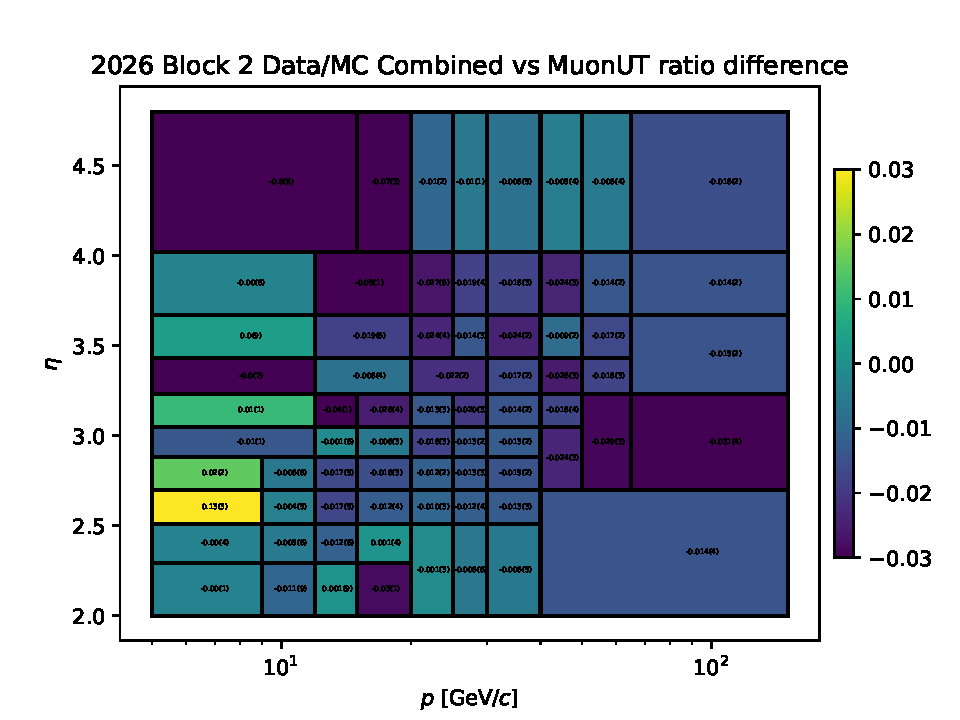
\includegraphics[width=0.85\textwidth]{Plots/TrackingEfficiencies_2D_binning_2026_Block2_RatioDiff_colour.pdf}
  \end{figure}
\end{frame}

\begin{frame}{Summary}
  \vspace{0.0cm}
  {\large We have prepared 2026 tracking efficiency tables, but:}
  \vspace{0.2cm}
  \begin{itemize}
    \setlength\itemsep{1.0em}
    \item{Expected 2026 MC is used}
    \item{Large discrepancies in SciFi seen, possibly due to radiation damage}
    \item{Issues with Velo efficiencies at high and low $\eta$ to be understood}
    \item{Feedback/comments welcome!}
  \end{itemize}
\end{frame}

\begin{frame}{Next steps}
  \vspace{0.0cm}
  {\large Currently working on a new release of 2024 efficiencies:}
  \begin{enumerate}
    \item{Larger MC sample}
    \item{Separate corrections for $\mu^\pm$, $\mu^+$, $\mu^-$}
    \item{New 2D binning}
  \end{enumerate}
  \vspace{0.1cm}
  \begin{center}
    \Huge Thanks for your attention!
  \end{center}
\end{frame}

\begin{frame}{Backup}
  \vspace{0.0cm}
  \begin{center}
    \huge Backup
  \end{center}
\end{frame}

\begin{frame}{2026 tracking efficiency ratios}
  \vspace{0.0cm}
  {\large Comparison of tracking efficiency ratios in 2026 Block 3}
  \begin{figure}[htb]
    \centering
    \begin{subfigure}{0.5\textwidth}
      \centering
      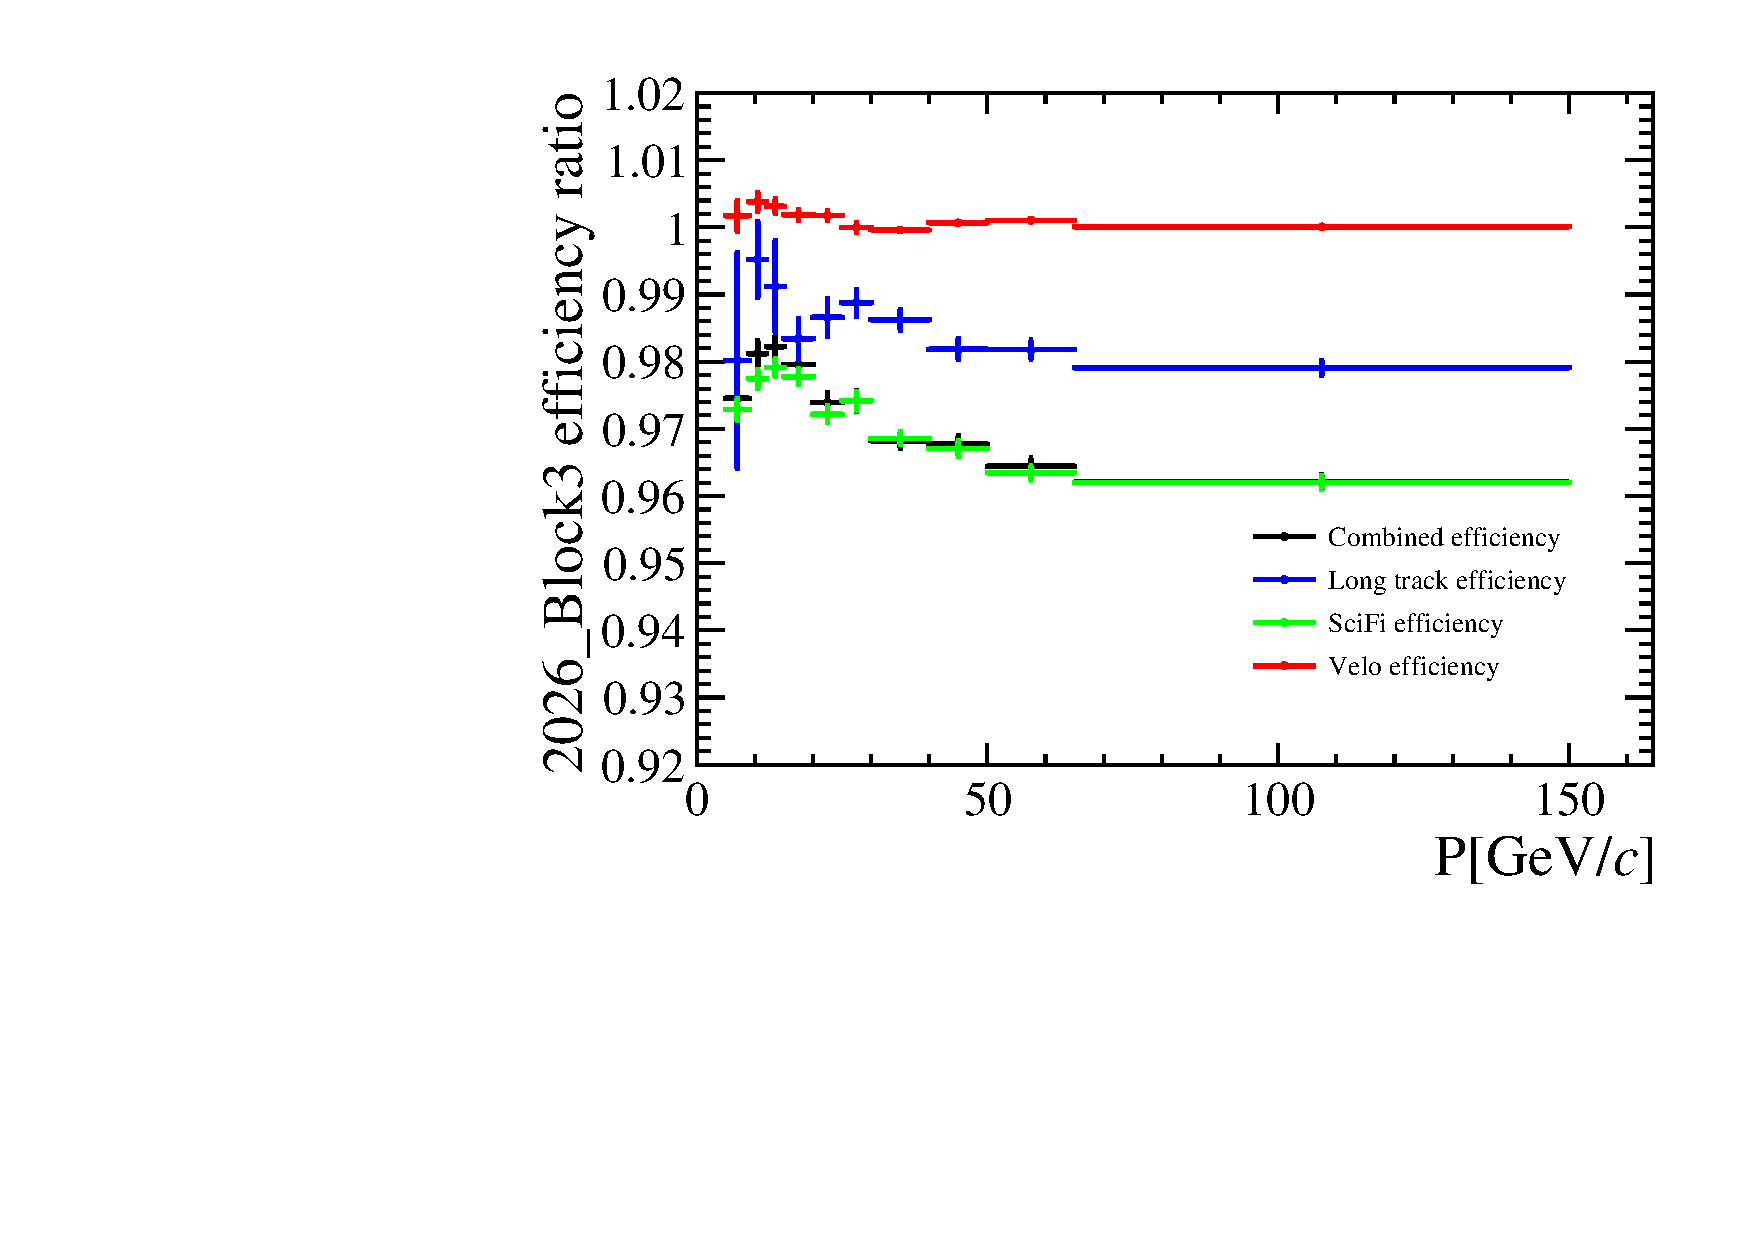
\includegraphics[width=1.0\textwidth]{Plots/trackeff_ratio_P_2026_Block3_2026_expected_MC_samples.pdf}
    \end{subfigure}%
    \begin{subfigure}{0.5\textwidth}
      \centering
      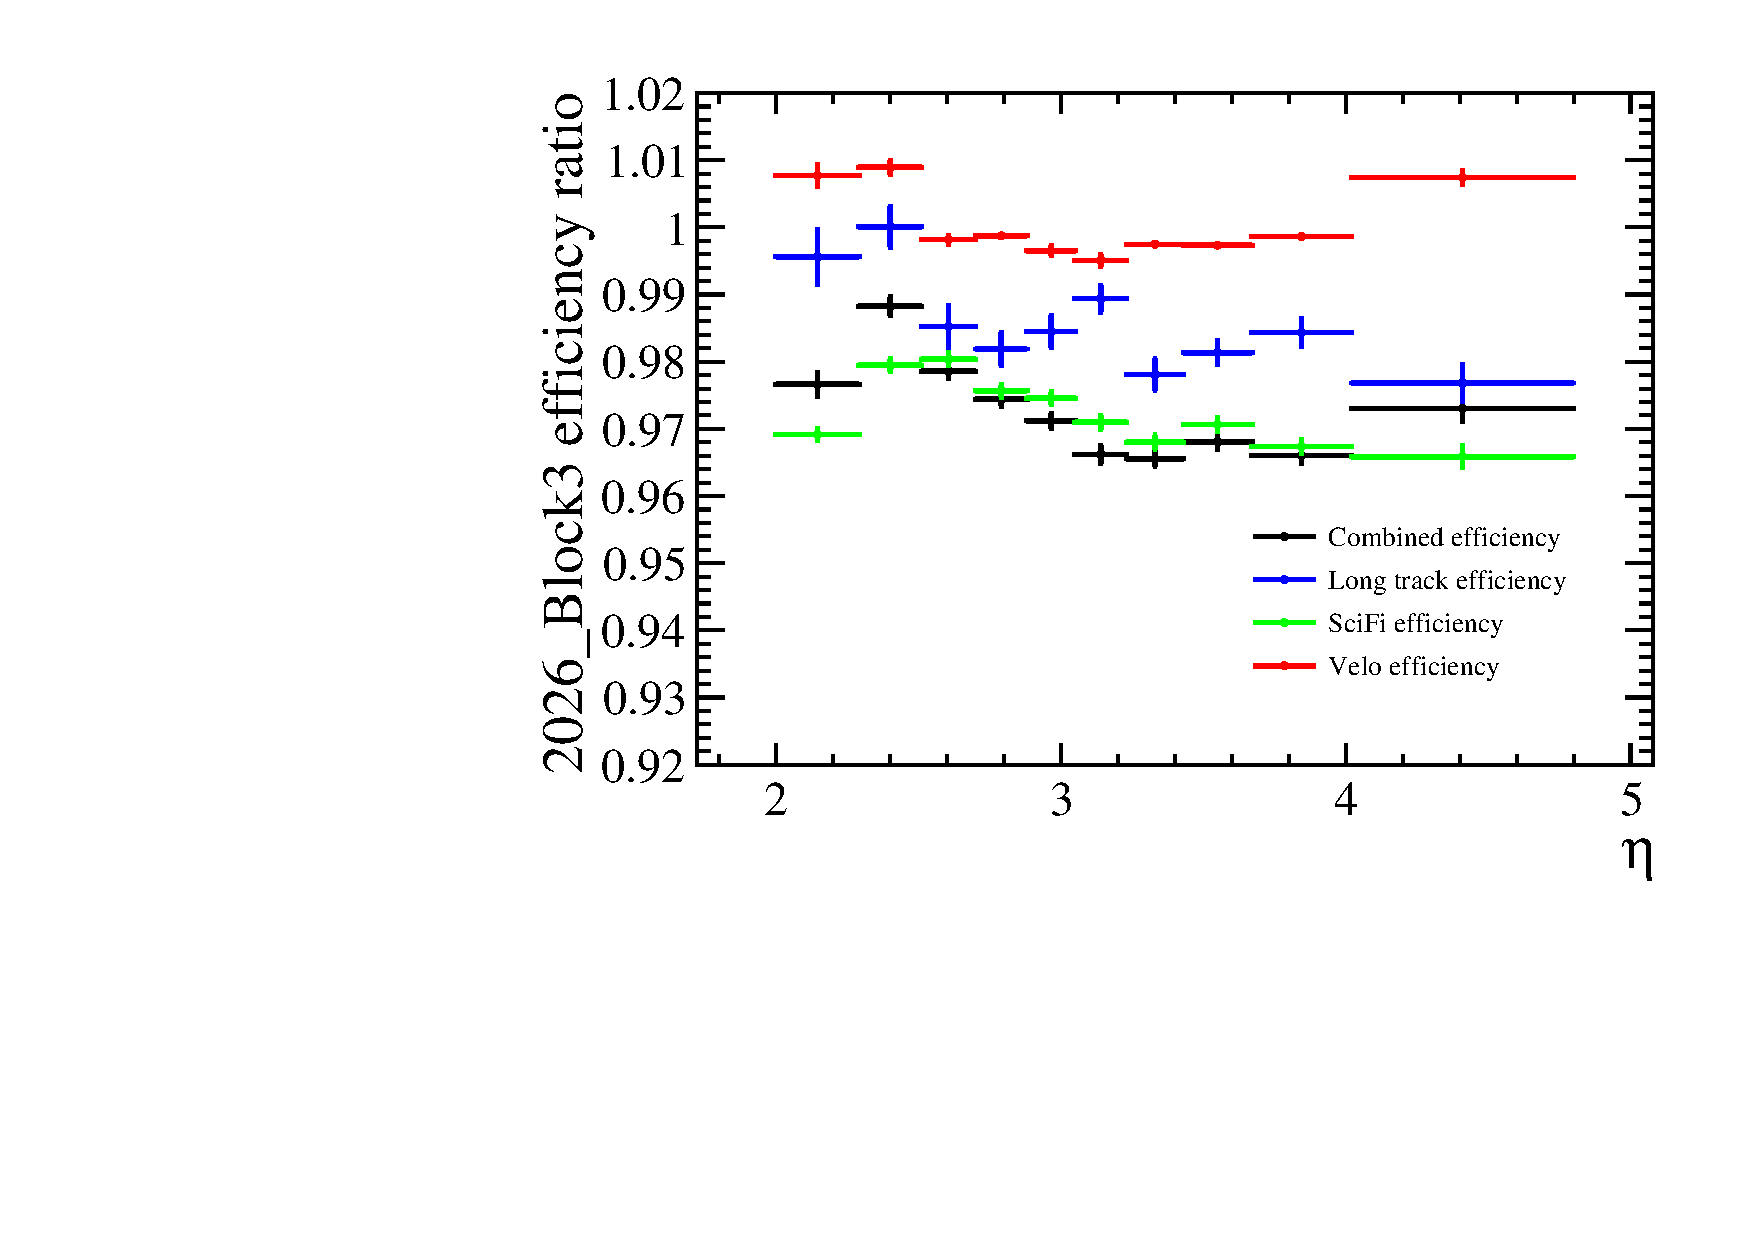
\includegraphics[width=1.0\textwidth]{Plots/trackeff_ratio_ETA_2026_Block3_2026_expected_MC_samples.pdf}
    \end{subfigure}
  \end{figure}
  {2026 Block 3 shows some discrepancies in Velo efficiencies}
\end{frame}

\begin{frame}{2026 tracking efficiency ratios}
  \vspace{0.0cm}
  {\large Comparison of tracking efficiency ratios in 2026 Block 4}
  \begin{figure}[htb]
    \centering
    \begin{subfigure}{0.5\textwidth}
      \centering
      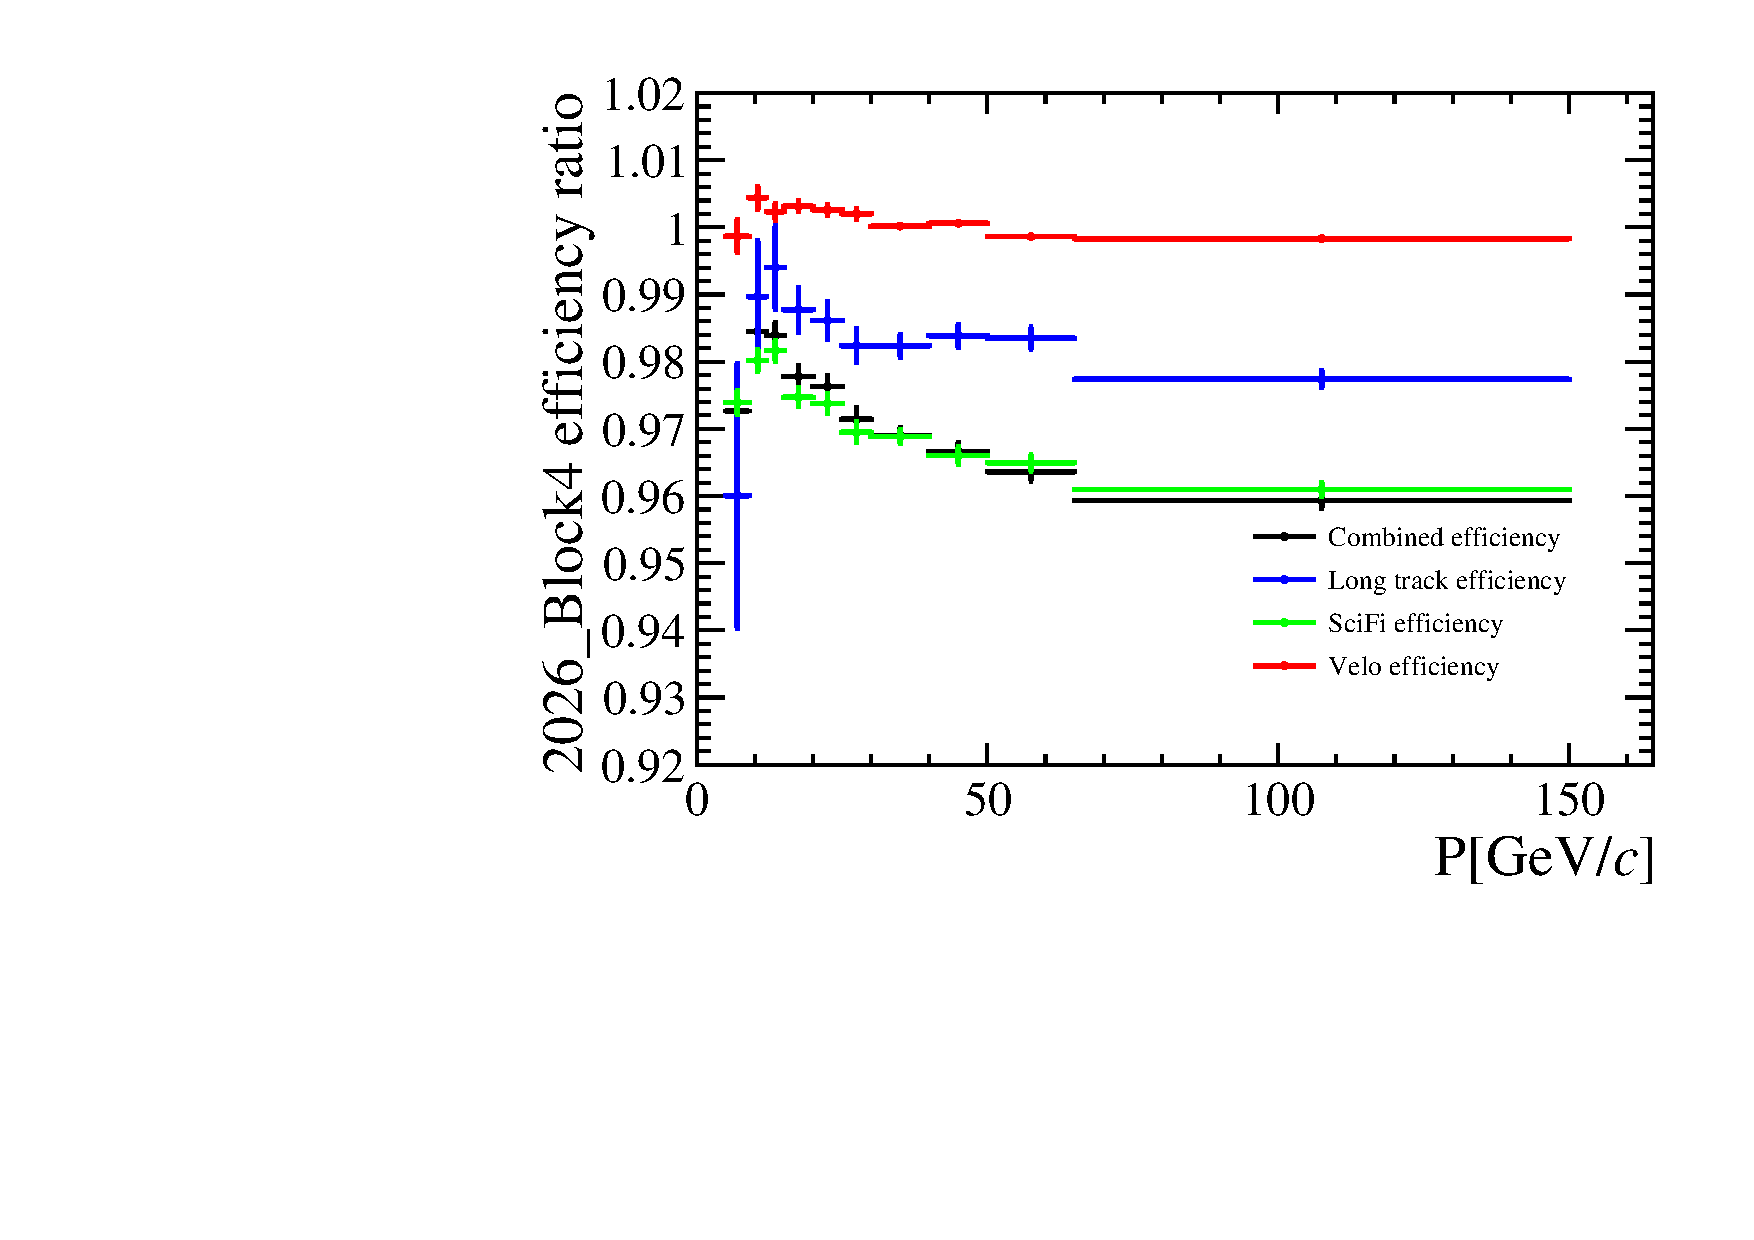
\includegraphics[width=1.0\textwidth]{Plots/trackeff_ratio_P_2026_Block4_2026_expected_MC_samples.pdf}
    \end{subfigure}%
    \begin{subfigure}{0.5\textwidth}
      \centering
      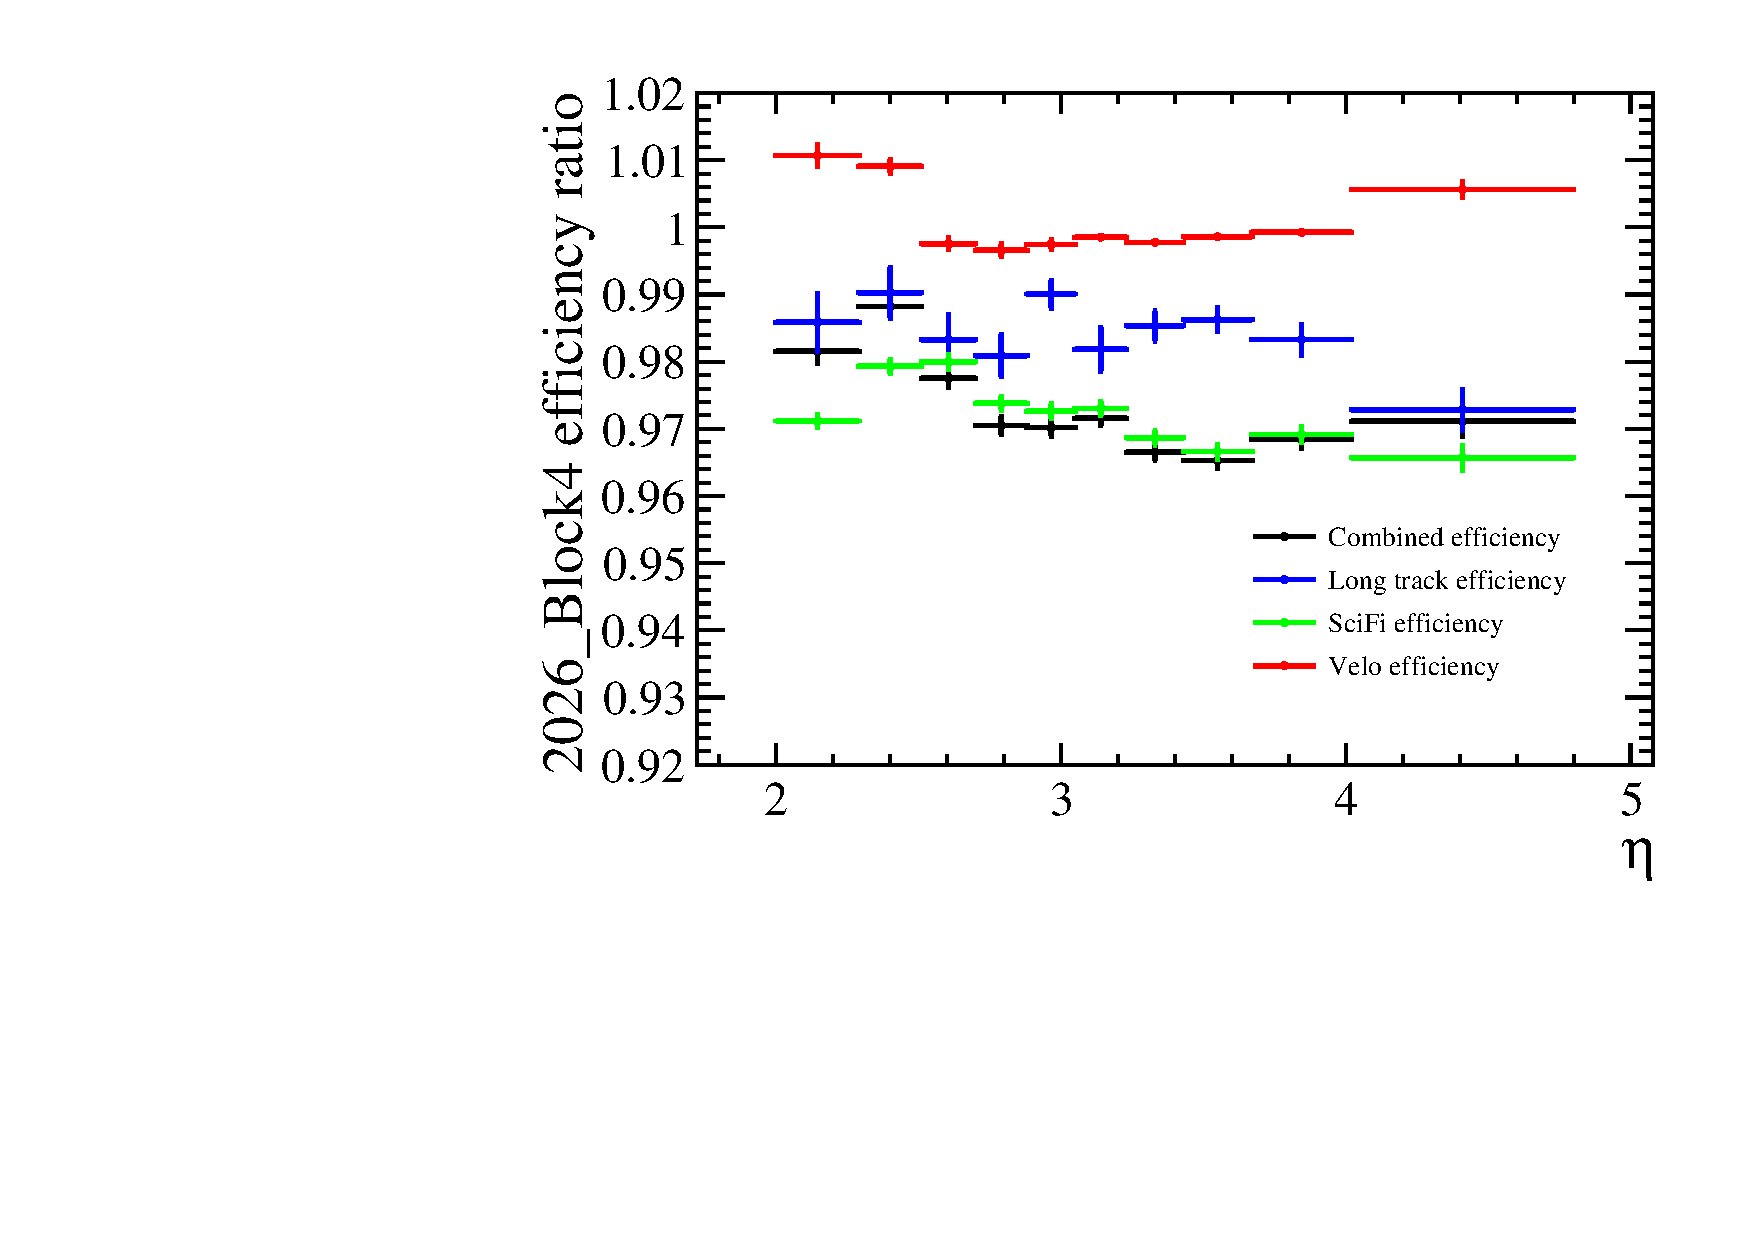
\includegraphics[width=1.0\textwidth]{Plots/trackeff_ratio_ETA_2026_Block4_2026_expected_MC_samples.pdf}
    \end{subfigure}
  \end{figure}
  {2026 Block 4 shows some discrepancies in Velo efficiencies}
\end{frame}

\end{document}
